\documentclass[twoside,11pt]{article}
\usepackage[mathscr]{euscript}
\usepackage{algorithmic}
\usepackage{algorithm}
\usepackage{amsfonts}
\usepackage{amsmath}
\usepackage{amssymb}
\usepackage{amstext}
\usepackage{bm}
\usepackage{caption}
\usepackage{color}
\usepackage{dsfont}
\usepackage{enumerate}
\usepackage{graphicx}
\usepackage{jmlr2e}
\usepackage{latexsym}
\usepackage{multirow}
\usepackage{natbib}
\usepackage{upgreek}
\usepackage{url}
\usepackage{hyperref}
\newcommand{\ignore}[1]{}
\setcounter{tocdepth}{3}
\usepackage{lastpage}

%\let\doendproof\endproof
%\renewcommand\endproof{~\hfill\qed\doendproof}

%\setlength{\parskip}{-0.01cm}
%\def\baselinestretch{0.92}

\def\Rset{\mathbb{R}}
\def\Hset{\mathbb{H}}
\def\Nset{\mathbb{N}}
\DeclareMathOperator*{\E}{\rm E}
\DeclareMathOperator*{\argmax}{\rm argmax}
\DeclareMathOperator*{\argmin}{\rm argmin}
\DeclareMathOperator{\sgn}{sgn}
\DeclareMathOperator{\supp}{supp}
\DeclareMathOperator{\rank}{rank}
\DeclareMathOperator{\diag}{diag}
\DeclareMathOperator{\last}{last}
\DeclareMathOperator{\Tr}{Tr}
\providecommand{\abs}[1]{\lvert#1\rvert}
\providecommand{\norm}[2]{\lVert#1\rVert_{#2}}
\providecommand{\frob}[2]{\langle#1, #2\rangle_F}

\newcommand{\e}{\epsilon}
\newcommand{\h}{\widehat}
\newcommand{\wt}{\widetilde}

\newcommand{\new}{\marginpar{NEW}}
\newcommand{\nqed}{\hfill\nopagebreak\mbox{}\hfill\qed}
\newcommand{\parenthesize}[1]{\left( #1 \right)}
\newcommand{\set}[1]{\{#1\}}
\newcommand{\tts}{\tt \small}
\newcommand{\Span}{\operatorname{span}}

\newcommand{\cA}{{\mathcal A}}
\newcommand{\cD}{{\mathcal D}}
\newcommand{\cF}{{\mathcal F}}
\newcommand{\cH}{{\mathcal H}}
\newcommand{\cL}{{\mathcal L}}
\newcommand{\cQ}{{\mathcal Q}}
\newcommand{\cS}{{\mathcal S}}
\newcommand{\cT}{{\mathcal T}}
\newcommand{\cX}{{\mathcal X}}
\newcommand{\cY}{{\mathcal Y}}

\newcommand{\mat}[1]{{\mathbf #1}}
\renewcommand{\P}{\mat{\Phi}}
\renewcommand{\a}{\mat{a}}
\renewcommand{\b}{\mat{b}}
\newcommand{\1}{\mat{1}}
\newcommand{\bu}{\mat{u}}
\newcommand{\bv}{\mat{v}}
\newcommand{\bq}{\mat{q}}
\newcommand{\Ks}{\mat{K}_s}
\newcommand{\Kst}{\mat{K}_{st}}
\newcommand{\Kt}{\mat{K}_{t}}
\renewcommand{\v}{\mat{v}}
\newcommand{\w}{\mat{w}}
\newcommand{\x}{\mat{x}}
\newcommand{\y}{\mat{y}}
\newcommand{\z}{\mat{z}}
\newcommand{\I}{\mat{I}}
\newcommand{\X}{\mat{X}}
\newcommand{\W}{\mat{W}}
\newcommand{\Z}{\mat{Z}}

\newcommand{\qq}{{\mathsf q}}
\newcommand{\QQ}{{\mathsf Q}}
\newcommand{\uu}{{\mathsf u}}
\newcommand{\UU}{{\mathsf U}}

\newcommand{\m}{\mathfrak{m}}
\newcommand{\n}{\mathfrak{n}}
\newcommand{\q}{\mathfrak{q}}
\newcommand{\R}{\mathfrak{R}}

\newcommand{\qmin}{{\qq_\text{min}}}
\newcommand{\qpmin}{{\qq'_\text{min}}}
\newcommand{\adapt}{\text{adapt}}
\newcommand{\Alpha}{{\boldsymbol \alpha}}
\newcommand{\Beta}{{\boldsymbol \beta}}
\newcommand{\Br}{B_r}
\newcommand{\dis}{\mathrm{disc}}
\newcommand{\DIS}{\mathrm{DISC}}
\newcommand{\fix}{\marginpar{FIX}}
\newcommand{\llambda}{{\boldsymbol \lambda}}
\newcommand{\Rad}{\mathfrak{R}}
%\newcommand{\dinf}{d_{\infty | \supp(\h P)}}
\newcommand{\dinf}{\h d_\infty}
\newcommand{\dbar}{\overline d}
\newcommand{\done}{d_1}

%\newtheorem{proposition}{Proposition}
%\newtheorem{lemma}{Lemma}
%\newtheorem{corollary}{Corollary}
%\newtheorem{theorem}{Theorem}
%\newtheorem{definition}{Definition}

\makeatletter
\renewcommand{\@listI}{%
\leftmargin=20pt
\rightmargin=0pt
\labelsep=5pt
\labelwidth=20pt
\itemindent=0pt
\listparindent=0pt
\topsep=0pt plus 3pt
\partopsep=0pt plus 3pt
\parsep=0pt plus 1pt
\itemsep=\parsep}
\makeatother

\hypersetup{
  colorlinks   = true, %Colors links instead of ugly boxes
  urlcolor     = black, %Colour for external hyperlinks
  linkcolor    = black, %Colour of internal links
  citecolor   = black %Colour of citations
}

% \jmlrheading{20}{2019}{1-\pageref{LastPage}}{10/17}{1/19}{17-608}{all
% authors FULL names}

\jmlrheading{20}{2019}{1-\pageref{LastPage}}{5/15; Revised 10/15}{1/19}{15-192}{Corinna Cortes, Mehryar Mohri, Andr\'es Mu\~noz Medina}
\ShortHeadings{Adaptation Based on Generalized Discrepancy}{Cortes, Mohri and Mu\~noz Medina}

\begin{document}

\title{Adaptation Based on Generalized Discrepancy}

\author{Corinna Cortes {\email corinna@google.com} \\
\addr Google Research,  111 8th ave, New York, NY 10011
\AND
Mehryar Mohri {\email mohri@cims.nyu.edu} \\
Andr\'es Mu\~noz Medina {\email munoz@cims.nyu.edu} \\
\addr Courant Institute of Mathematical Sciences,
251 Mercer Street,
New York, NY 10012
}

\editor{Multi Task Learning}

\maketitle

\begin{abstract} %

We present a new algorithm for domain adaptation improving upon a
discrepancy minimization algorithm, (DM), previously shown to
outperform a number of algorithms for this problem. Unlike many
previously proposed solutions for domain adaptation, our algorithm does
not consist of a fixed reweighting of the losses over the training
sample. Instead, the reweighting depends on the hypothesis sought.
The algorithm is derived from a less conservative notion of
discrepancy than the DM algorithm called
\emph{generalized discrepancy}. We present a detailed description of
our algorithm and show that it can be formulated as a convex
optimization problem. We also give a detailed theoretical analysis of
its learning guarantees which helps us select its parameters.
Finally, we report the results of experiments demonstrating that it
improves upon discrepancy minimization.

\end{abstract}
\begin{keywords}
domain adaptation, learning theory
\end{keywords}

\section{Introduction}

A standard assumption in statistical learning theory and PAC learning
is that training and test samples are drawn from the same distribution
\citep{Vapnik1998,Valiant1984}. In practice, however, this assumption
often does not hold: the source and target distributions may somewhat
differ. This problem is known as \emph{domain adaptation} and
arises in a variety of applications such as natural language
processing and computer vision
\citep{Dredze07Frustratingly,Blitzer07Biographies,jiang-zhai07,
  LegetterWoodlang,\ignore{Rosenfeld96,}Martinez2002,HoffmanDarrellSaenko2014}. The
domain adaptation problem may appear when the distributions over
the instance space differ, the so-called \emph{covariate shift}
problem, or when the labeling functions associated with each
domain disagree. In practice, a combination of both issues occurs and,
for adaptation to succeed, the divergence between the two domains
needs to be relatively small. This is clear for the labeling functions
since, if the learner receives source labels that are vastly different
from the target ones, no learning algorithm can generalize
well to the target domain. The same holds when input distributions
largely differ.

This intuition was formalized by \cite{shai2010} and
\cite{BenDavidUrner2012} who showed that even in the favorable
scenario where the source and target distribution admit the same
support, a sample of size in the order of that of the support is
needed in order to solve the domain adaptation problem. As the authors
point out, the domain adaptation problem becomes intractable when the
labeling function for the training data is vastly different from the
labeling function used for testing. On the other hand, when some
similarity between domains exist, it has been empirically and
theoretically shown that adaptation algorithms can be
beneficial and in fact a large number of algorithms for this task have
been proposed over the past decade. The large majority of them fall in
one of the following paradigms:

\begin{enumerate}
\item {\bf Learning a new feature representation}. The core idea behind
these algorithms is to map the source and target data into a new
feature space where the difference between source and target
distributions is reduced. Transfer Component Analysis (TCA)
\citep{PanTKY11} and the work on Frustratingly Easy Domain Adaptation
(FE) \citep{daume2007frustratingly} belong to this family of
algorithms. Whereas some empirical evidence of the effectiveness of
these algorithms exists in the literature, to the best of our
knowledge, no work has been done to provide learning guarantees for
these algorithms.

\item {\bf Reweighting}. Originated in the Statistics literature on
sample bias correction, these techniques attempt to correct the
difference between distributions by multiplying the loss at each
training example by a positive weight. Most of the classical
algorithms such as KMM
\citep{HuangSmolaGrettonBorgwardtScholkopf2006}, KLIEP \citep{
SugiyamaNakajimaKashimaVonBunauKawanabe2008} and a two-step algorithm
by \cite{BickelBrucknerScheffer2007} fall in this category.
\end{enumerate}

The main focus of this work will be on the latter. A common trait
shared by most algorithms in this category is that their reweighting
schemes are based on the minimization of a divergence measure between
the empirical source and target distributions. For instance, the
KL-divergence in the case of KLIEP and the Maximum Mean Discrepancy
(MMD) \citep{GrettonMMD} for KMM. The guarantees of these algorithms
are therefore given as a function of the chosen divergence. The main
drawback of these measures is that they do not take into account the
hypothesis set or the loss function, both crucial components of any
learning algorithm. In contrast, the \emph{discrepancy} introduced by
\cite{MansourMohriRostamizadeh2009} and further studied by
\cite{CortesMohri2011} is a measure of the divergence between
distributions tailored to domain adaptation that precisely takes into
account both the loss function and the hypothesis set.  The
$d_\cA$-distance, introduced by
\cite{DevroyeGyorfiLugosi1996}[pp. 271-272] under the name of
\emph{generalized Kolmogorov-Smirnov distance}, later by
\cite{BenDavidBlitzerCrammerPereira2006}, coincides with the
discrepancy when the binary loss function is used.  The discrepancy is
a pivotal concept used in the analysis of several adaptation
scenarios:  the $\cY$-discrepancy or \emph{integral
  probability metric} \citep{ZhangZhangYe2012} was successfully used
by \cite{drift}
to provide tight learning guarantees for the related task of learning
with drifting distributions, whereas a modified version of the
discrepancy was used by \cite{germain2013pac} to study the problem of
domain adaptation in a PAC-Bayesian setting. The discrepancy-based
generalization bounds given by \cite{MansourMohriRostamizadeh2009}
motivated a discrepancy minimization (DM) algorithm
\citep{CortesMohri2013}, which attempts to minimize said
bounds. Besides its favorable theoretical guarantees, this algorithm
was shown to perform well in a number of adaptation tasks and to match
or outperform several other algorithms such as KMM, KLIEP and the
aforementioned two stage algorithm by
\citet{BickelBrucknerScheffer2007}.

One shortcoming of the DM algorithm, however, is that it seeks to
reweight the loss on the training samples to minimize a quantity
defined as the maximum over \emph{all} pairs of hypotheses, including
hypotheses that the learning algorithm might not ever consider as
candidates. Thus, the algorithm tends to be too conservative on its
choice of weights. We present an alternative theoretically well
founded algorithm for domain adaptation that is based on minimizing a
finer quantity, the \emph{generalized discrepancy}, and that seeks to
improve upon DM.  Unlike the DM algorithm, our algorithm does not
consist of a \emph{fixed} reweighting of the losses over the training
sample. Instead, the weights assigned to training sample losses vary
as a function of the hypothesis $h$. This helps us ensure that for
every hypothesis, $h$, the empirical loss on the source distribution
is as close as possible to the empirical loss on the target
distribution for that particular $h$.

We describe the learning scenario considered
(Section~\ref{sec:scenario}), then present a detailed description of
our algorithm and show that it can be formulated as a convex
optimization problem (Section~\ref{sec:algorithm}). Next, we analyze
the theoretical properties of our algorithm, which guide us in
choosing the surrogate hypothesis set defining our algorithm
(Section~\ref{sec:guarantees}). In Section~\ref{sec:optimization}, we
further analyze the optimization problem defining our algorithm and
derive an equivalent form that can be handled by a standard convex
optimization solver.  In Section~\ref{sec:experiments}, we report the
results of experiments demonstrating that our algorithm improves upon
the DM algorithm in several tasks.

\section{Learning Scenario}
\label{sec:scenario}

This section defines the learning scenario of domain adaptation we
consider, which coincides with that of
\cite{BenDavidBlitzerCrammerPereira2006} or
\cite{MansourMohriRostamizadeh2009,CortesMohri2013}. We
first introduce the definitions and concepts needed for the following
sections. For the most part, we follow the definitions and notation of
\citet{CortesMohri2013}.

Let $\cX$ denote the input space and $\cY \subseteq \Rset$ the output
space. We define a \emph{domain} as a pair formed by a distribution
over $\cX$ and a target labeling function mapping from $\cX$ to
$\cY$. Throughout the paper, $(Q, f_Q)$ denotes the \emph{source
domain} and $(P, f_P)$ the \emph{target domain} with $Q$ the source
and $P$ the target distribution over $\cX$ and with
$f_Q, f_P \colon \cX \to \cY$ the source and target labeling
functions, respectively.

In the scenario of \emph{domain adaptation} we consider, the learner
receives two samples: a labeled sample of $m$ points from the source
domain $\cS = ((x_1,y_1), \ldots, (x_m, y_m)) \in (\cX \times \cY)^m$
with $x_1, \ldots, x_m$ drawn i.i.d.\ according to $Q$ and
$y_i = f_Q(x_i)$ for $i \in [1, m]$; and an unlabeled sample
$\cT = (x'_1, \ldots, x'_n)\in \cX^n$ of size $n$ drawn i.i.d.\
according to the target distribution $P$. We denote by $\h Q$ the
empirical distribution corresponding to the (unlabeled) sample
$\cS_\cX = (x_1, \ldots, x_m)$ and by $\h P$ the empirical
distribution corresponding to $\cT$. We will be in fact more
interested in the scenario commonly encountered in practice where, in
addition to these two samples, the learner receives a small amount of
labeled data
$\cT' = ((x''_1, y''_1), \ldots, (x''_{s}, y''_{s})) \in (\cX \times \cY)^{s}$
from the target domain.

We consider a loss function $L\colon \cY \times \cY \to \Rset_+$
jointly convex in its two arguments.  The $L_p$ losses commonly used
in regression and defined by $L_p(y, y') = |y' - y|^p$ for $p \geq 1$
are special instances of this definition.  For any two functions
$h, h'\colon \cX \to \cY$ and any distribution $D$ over $\cX$, we denote
by $\cL_D(h, h')$ the expected loss of $h(x)$ and
$h'(x)$: $\cL_D(h, h') = \E_{x \sim D} [L(h(x), h'(x))]$.  The
learning problem consists of selecting a hypothesis $h$ out of a
hypothesis set $H$ with a small expected loss $\cL_P(h, f_P)$ with
respect to the target domain.  We further extend this notation to
arbitrary functions $\qq\colon \cX \to \Rset$ with a finite support as
follows:
$\cL_\qq(h, h') = \sum_{x \in \cX} q(x) L(h(x), h'(x))$.

\begin{table}[t]
\centering
\begin{tabular}{|c|c||c|c|}
\hline
$\scriptstyle{\cX}$ & \small{Input space} & $\scriptstyle{\cY}$ & \small{Output space} \\
$\scriptstyle{P}$ & \small{Target distribution} & $\scriptstyle{Q}$ & \small{Source distribution} \\
$\scriptstyle{\h P} $ & \small{Empirical target distribution} & $\scriptstyle{\h Q}$ & \small{Empirical source distribution} \\
$\scriptstyle{\cT}$ & \small{Target unlabeled sample} & $\scriptstyle{ \cS}$ & \small{Labeled source sample} \\
$\scriptstyle{\cT'}$ & \small{Small target labeled sample} & $\scriptstyle{ \cS_\cX }$ &  \small{Unlabeled source sample} \\
$\scriptstyle{f_P}$ & \small{Target labeling function} & $\scriptstyle{f_Q}$ & \small{Source labeling function} \\
$\scriptstyle{\cL_{P}(h, f_P)}$ & \small{Expected target loss} & $\scriptstyle{\cL_{Q}(h, f_Q)}$ & \small{Expected source loss} \\
$\scriptstyle{\cL_{\h P}(h, f_P)}$ & \small{Empirical target loss} & $\scriptstyle{\cL_{\h Q}(h, f_Q)}$ & \small{Empirical source loss} \\
$\scriptstyle{\dis(P, Q)}$ & \small{Discrepancy} & $\scriptstyle{\DIS(\h P, \UU) }$ & \small{Generalized discrepancy} \\
$\scriptstyle{\dis_{H''}(P, Q)}$ & \small{Local Discrepancy} & $\scriptstyle{\dis_{\cY}(P, Q) }$ & $\scriptstyle{\cY}$\small{-discrepancy} \\
$\scriptstyle{\qmin}$ & \small{DM solution} & $\scriptstyle{\QQ_h}$ & \small{GDM solution }
 \\
\hline
\end{tabular}
\caption{Notation table.}
\label{table:notation}
\end{table}

\section{Algorithm}
\label{sec:algorithm}

In this section, we describe our new adaptation algorithm. We first
review some related previous work. Next, we present the key idea
behind our algorithm and derive its general form, and finally,
formulate it as a convex optimization problem.

\subsection{Previous Work}
\label{subsec:discmin}

It was shown by \citet{MansourMohriRostamizadeh2009} and
\citet{CortesMohri2011} (see also the \emph{$d_{\cA}$-distance}
\citep{BenDavidBlitzerCrammerPereira2006} in the case of binary loss
for classification) that a key measure of the difference of two
distributions in the context of adaptation is the
\emph{discrepancy}. Given a hypothesis set $H$, the discrepancy,
$\dis$, between two distributions $P$ and $Q$ over $\cX$ is defined
by:
\begin{equation}
 \dis(P, Q) = \max_{h, h' \in H} \big| \cL_{P}(h', h) - \cL_{Q}(h', h) \big|.
\end{equation}
The discrepancy has several advantages over other common divergence
measures such as the $L_1$ distance. We refer the reader to
\citep{thesis} for a detailed discussion on this subject.
Several generalization bounds for adaptation in terms of the
discrepancy have been given in the past
\citep{BenDavidBlitzerCrammerPereira2006,
MansourMohriRostamizadeh2009,CortesMohri2011,CortesMohri2013}.
including pointwise guarantees in the case of kernel-based
regularization algorithms, which includes algorithms such as support
vector machines (SVM), kernel ridge regression, or support vector
regression (SVR). The bounds given in
\citep{MansourMohriRostamizadeh2009} motivated a \emph{discrepancy
minimization} algorithm. Given a positive semi-definite (PSD) kernel
$K$, the hypothesis returned by the algorithm is the solution of the
following optimization problem
\begin{equation}
\label{eq:qmin-opt}
\min_{h \in \Hset} \quad \lambda \| h \|_K^2 + \cL_{\qmin} (h, f_Q),
\end{equation}
where $\| \cdot \|_K $ is the norm in the reproducing Hilbert space
$\Hset$ induced by the kernel $K$ and $\qmin$ is a distribution over
the support of $\h Q$ such that
$\qmin = \argmin_{\qq \in \cQ} \dis(\qq, \h P)$, where
$\cQ = [0,1]^{\cS_\cX}$ is the set of all distributions defined
over the support of $\h Q$. Besides its theoretical motivation, this
algorithm has been shown
to outperform several other algorithms in a series of experiments
carried out by \cite{CortesMohri2013}.

Observe that, by definition, the objective function optimized by
$\qmin$ corresponds to a maximum over all pairs of hypotheses. But,
the maximizing pair of hypotheses may not be among the candidates ever
considered by the learning algorithm. Thus, a learning algorithm based
on discrepancy minimization tends to be too conservative.

\subsection{Main Idea}
\label{sec:mainidea}

From here on we assume the algorithm selected by the learner is an
instance of a regularized risk minimization algorithm over the Hilbert
space $\Hset$ induced by a PSD kernel $K$. With knowledge of the
target labels, these algorithms return a hypothesis $h^*$ solution of
$\min_{h \in \Hset} F(h)$ where
\begin{equation}
\label{eq:Pmin}
F(h) = \lambda \| h \|_K^2 + \cL_{\h P} (h, f_P),
\end{equation}
where $\lambda \geq 0$ is a regularization parameter.  Thus, $h^*$ can
be viewed as the \emph{ideal hypothesis}.

In view of that, we can formulate our objective, in the
\emph{presence} of a domain adaptation problem, as that of finding a
hypothesis $h$ whose loss $\cL_P(h, f_P)$ with respect to the target
domain is as close as possible to $\cL_P(h^*, f_P)$. To do so, we will
seek in fact a hypothesis $h$ that is as close as possible to $h^*$,
which would imply the closeness of the losses with respect to the
target domains.  We do not have access to $f_P$ and can only access
the labels of the training sample $\cS$. Thus, we must resort to using
in our objective function, instead of $\cL_{\h P} (h, f_P)$, a
reweighted empirical loss over the training sample $\cS$.  The main
idea behind our algorithm is to define, for any $h \in \Hset$, a
reweighting function
$\QQ_h\colon \cS_\cX = \set{x_1, \ldots, x_m} \to \Rset$ such that the
objective function $G$ defined for all $h \in \Hset$ by
\begin{equation}
\label{eq:qhmin}
 G(h) = \lambda \| h \|_K^2 + \cL_{\QQ_h} (h, f_Q)
\end{equation}
is uniformly close to $F$, thereby resulting in close
minimizers. Since the first term of \eqref{eq:Pmin} and
\eqref{eq:qhmin} coincide, the idea consists equivalently of seeking
$\QQ_h$ such that $\cL_{\QQ_h}(h, f_Q) $ and $\cL_{\h P}(h, f_P)$ be
as close as possible.  Observe that this departs from the standard
reweighting methods: instead of reweighting the training sample with
some fixed set of weights, we allow the weights to vary as a function
of the hypothesis $h$. Note that we have further relaxed the condition
commonly adopted by reweighting techniques that the weights must be
non-negative and sum to one.

Of course, searching for $\QQ_h$ to directly minimize
$|\cL_{\QQ_h}(h, f_Q) - \cL_{\h P}(h, f_P)|$ is in general not
possible since we do not have access to $f_P$, but it is instructive
to consider the imaginary case where the average loss
$\cL_{\h P}(h, f_P)$ is known to us for any $h \in \Hset$.
$\QQ_h$ could then be determined via
\begin{equation}
\label{eq:qh}
\QQ_h = \argmin_{\qq \in \cF(\cS_\cX, \Rset)} | \cL_\qq(h, f_Q) - \cL_{\h P}(h, f_P)|,
\end{equation}
where $\cF(\cS_\cX, \Rset)$ is the set of real-valued functions defined
over $\cS_\cX$. For any $h$, we can in fact select $\QQ_h$ such that
$\cL_{\QQ_h}(h, f_Q) = \cL_{\h P}(h, f_P)$ since $\cL_\qq(h, f_Q)$ is
a linear function of $\qq$. Thus, the optimization problem
\eqref{eq:qh} reduces to solving a simple linear equation. With this
choice of $\QQ_h$, the objective functions $F$ and $G$ coincide and by
minimizing $G$ we can recover the ideal solution $h^*$.  Note that, in
general, the DM algorithm could not recover that ideal solution. Even
a finer discrepancy minimization algorithm exploiting the knowledge of
$ \cL_{\h P}(h, f_P)$ for all $h$ and seeking a distribution
$\qq'_\text{min}$ minimizing
$\max_{h \in H} | \cL_\qq(h, f_Q) -\cL_{\h P}(h, f_P)|$ could not, in
general, recover the ideal solution since we could not have
$\cL_{\qq'_\text{min}}(h, f_Q) = \cL_{\h P}(h, f_P)$ for all
$h \in \Hset$.

Of course, $\cL_{\h P}(h, f_P)$ is not accessible since the sample
$\cT$ is unlabeled. Instead, we will consider a non-empty convex set
of candidate hypotheses $H'' \subseteq H$ that could contain a good
approximation of $f_P$. Using $H''$ as a set of surrogate labeling
functions leads to the following definition of $\QQ_h$ instead of
\eqref{eq:qh}:
\begin{equation}
\label{eq:agnosqh}
\QQ_h = \argmin_{\qq \in \cF(\cS_\cX, \Rset)} \max_{h'' \in H''}|
\cL_\qq(h, f_Q) - \cL_{\h P}(h, h'') |.
\end{equation}
The choice of the subset $H''$ is of course key. Our choice will be
based on the theoretical analysis of
Section~\ref{sec:guarantees}. Nevertheless, we now
present the formulation of the optimization problem for an
arbitrary choice of the convex subset $H''$.

\begin{proposition}
\label{prop:maxmin}
For any $h \in \Hset$, let $\QQ_h$ be defined by \eqref{eq:agnosqh}.
Then, the following identity holds for any $h \in \Hset$:
\begin{equation*}
  \cL_{\QQ_h}(h, f_Q) = \frac{1}{2} \Big(\max_{h'' \in H''} \cL_{\h
    P}(h, h'') + \min_{h'' \in H''}\cL_{\h P}(h, h'') \Big).
\end{equation*}
\end{proposition}

\begin{proof}
  For any $h \in \Hset$, the equation
$\cL_{\bq}(h, f_Q) =  l$ with $l \in \Rset$ admits a solution
$\qq \in \cF(\cS_\cX,  \Rset)$. Thus,
$\{\cL_{\qq}(h, f_Q) : \qq \in \cF(\cS_\cX, \Rset)\}  = \Rset$
and for any $h \in \Hset$, we can write
\begin{align*}
\cL_{\QQ_h}(h, f_Q)
& = \argmin_{\substack{l \in \set{\cL_{\bq}(h, f_Q)\colon \qq \in
      \cF(\cS_\cX, \Rset)}}} \max_{h'' \in H''}| l - \cL_{\h P}(h, h'')| \\
& = \argmin_{l \in \Rset} \max_{h'' \in H''}| l - \cL_{\h P}(h, h'') | \\
& = \argmin_{l \in \Rset} \max_{h''\in H''} \max \Big \{ \cL_{\h P}(h, h'')
  - l, l - \cL_{\h P}(h, h'') \Big \}\\
& = \argmin_{l \in \Rset} \max \Big \{ \max_{h''\in H''} \cL_{\h P}(h, h'')
  - l, l - \min_{h''\in H'' } \cL_{\h P}(h, h'') \Big \}\\
& = \frac{1}{2} \Big(\max_{h'' \in H''} \cL_{\h
    P}(h, h'') + \min_{h'' \in H''}\cL_{\h P}(h, h'') \Big),
\end{align*}
since the minimizing $l$ is obtained for
$\displaystyle \!\!\max_{h''\in H''} \cL_{\h P}(h,h'') - l
\!=\! l - \!\!\min_{h''\in H'' }\cL_{\h P}(h, h'')$.
\end{proof}

In view of this proposition, with our choice of $\QQ_h$ based on
\eqref{eq:agnosqh}, the objective function $G$ of our algorithm
\eqref{eq:qhmin} can be equivalently written for all $h \in \Hset$ as
follows:
\begin{equation}
\label{eq:optmaxmin}
G(h) =  \lambda\| h \|_K^2 + \frac{1}{2} \Big(\max_{h'' \in
  H''} \cL_{\h P}(h, h'') + \min_{h'' \in H''}\cL_{\h P}(h, h'')\Big).
\end{equation}
Using the fact the $\cL_{\h P}$ is a jointly convex function, it is
easy to show (see for instance \citealp{BoydVandenberghe2004}) that $G$
is in fact a convex function too.

\section{Learning Guarantees}
\label{sec:guarantees}

Here, we present two different types of guarantees: a tight learning bound
based on the Rademacher complexity and a pointwise bound derived from a
stability analysis. We further show that our algorithm is in fact
minimizing this pointwise bound. As in previous work, we assume that
the loss function $L$ is \emph{$\mu$-admissible}.

\begin{definition}
A loss function $L$ is $\mu$-admissible if there exists
$\mu > 0$ such that the inequality
\begin{equation}
\label{eq:mu-admissible}
|L(h(x), y) - L(h'(x), y)| \leq \mu |h(x) - h'(x)|
\end{equation}
holds for all $(x, y) \in \cX \times \cY$ and $h', h \in H$.
\end{definition}

The $L_p$ losses commonly used in
regression, $p \geq 1$, verify this condition (see
Appendix~\ref{app:muadmissible}).

\subsection{Rademacher Complexity Bounds}
\label{sec:rademachercomplexitybound}

\begin{definition}
  Let $\mathcal Z$ be any set and $G$ be a family of functions mapping
$\mathcal{Z}$ to $\Rset$. Given a sample
$\mathcal{S} = \{z_1, \ldots,z_n \} \subset \mathcal Z$, the empirical
Rademacher complexity of $G$ is denoted by $\h \Rad_{\mathcal{S}}(G)$
and defined by
\begin{equation*}
\h \Rad_{\mathcal{S}}(G) = \frac{1}{n} \E_{\sigma} \bigg[ \sup_{g\in G}
 \sum_{i=1}^n \sigma_i g(z_i) \bigg],
\end{equation*}
where $\sigma_i$s, called Rademacher variables, are independent random
variables distributed according to the uniform distribution over
$\{-1, 1\}$.  The Rademacher complexity of $G$ is defined as
\begin{equation*}
  \Rad_n(G) = \E_{\mathcal{S}}\big[ \h \Rad_{\mathcal{S}}(G) \big].
\end{equation*}
\end{definition}

Our first generalization bound is given in terms of the
\emph{$\cY$-discrepancy}, which is a generalization of the discrepancy
distance. The $\cY$-discrepancy was first introduced by \cite{drift}
in the context of learning with drifting distributions.
\begin{definition}
  The $\cY$-discrepancy between two domains $(P, f_P)$ and $(Q, f_Q)$
  is defined by
\begin{equation*}
   \dis_\cY(P, Q) = \sup_{h \in H} \big| \cL_Q(h, f_Q) - \cL_P(h, f_P) \big|.
\end{equation*}
\end{definition}
Note that the definition depends on the labeling functions $f_P$ and
$f_Q$. We do not explicitly indicate that dependency for the sake of
simplicity of the notation.

We follow the analysis of \citep{drift} to derive the following tight
generalization bounds based on the notion of $\cY$-discrepancy.

\begin{proposition}
\label{prop:ydiscbounds}

Let $\cH_Q$ and $\cH_P$ be the families of functions defined as
follows: $\cH_Q := \{ x \mapsto L(h(x),f_Q(x)) \colon h \in H \}$ and
$\cH_P := \{ x \mapsto L(h(x), f_P(x)) \colon h \in H \}$. Define
$M_Q$ and $M_P$ as
$M_Q = \sup_{x \in \mathcal{X}, h \in H} L(h(x), f_Q(x))$ and
$M_P = \sup_{x \in \mathcal{X}, h \in H} L(h(x), f_P(x))$.
Then, for any $\delta > 0$,
\begin{enumerate}
\item with probability at least $1 - \delta$ over the choice of a
labeled sample $\cS$ of size $m$, the following inequality holds
for all $h \in H$:\\[-.4cm]
\begin{equation}
\label{eq:truedisclearning}
 \cL_{P} (h, f_P) \leq \cL_{\h Q}(h, f_Q) + \dis_\cY(P, Q)
+ 2 \Rad_m(\cH_Q) + M_Q \sqrt{\frac{\log(\frac{1}{\delta})}{2 m}};
\end{equation}
\item with probability at least $1 - \delta$ over the choice of a
  sample $\mathcal{T}$ of size $n$, the following inequality holds for
  all $h \in H$ and
  any distribution $\qq$ over a sample $\cS_{\cX}$:\\[-.4cm]
\begin{equation}
\label{eq:empdisclearning}
\cL_{P}(h, f_P) \leq \cL_{\qq}(h, f_Q)  + \dis_\cY(\h P, \qq)
 + 2 \Rad_n(\cH_P) + M_P \sqrt{\frac{\log(\frac{1}{\delta})}{2 n}}.
\end{equation}
\end{enumerate}
\end{proposition}

\begin{proof}
  Let $\Phi(\mathcal{S})$ denote
$\sup_{h \in H} \cL_{\h Q}(h, f_Q) -  \cL_{P}(h, f_P)$. Changing one
point in $\mathcal{S}$ changes $\Phi(\mathcal{S})$ by at most
$\frac{M_Q}{m}$. Thus, by McDiarmid's inequality, we have
$\mathbb{P} \big( \Phi(\mathcal{S}) - \E[\Phi(\mathcal{S})] > \e \big) \leq
e^{-\frac{2 m \epsilon^2}{M_Q^2}}$. Therefore, for any $\delta > 0$,
with probability at least $1 - \delta$, the following holds for all $h \in H$:
\begin{equation*}
 \cL_{P} (h, f_P) \leq \cL_{\h Q}(h, f_Q) + \E[\Phi(\mathcal{S})]  + M_Q
 \sqrt{\frac{\log(\frac{1}{\delta})}{2 m}}.
\end{equation*}
Next, we can bound $\E[\Phi(\mathcal{S})]$ as follows:
\begin{align*}
 \E[\Phi(\mathcal{S})]
& = \E\bigg[\sup_{h \in H} \cL_{\h Q}(h, f_Q) - \cL_P(h, f_P) \bigg] \\
& \leq \E\bigg[\sup_{h \in H} \cL_{\h Q}(h, f_Q) - \cL_{Q}(h, f_Q)\bigg]  +
\sup_{h \in H} \cL_Q(h, f_Q) - \cL_P(h, f_P) \\
&\leq 2 \Rad_m(\cH_Q) + \dis_\cY(P, Q),
\end{align*}
where the last inequality follows from a standard symmetrization
inequality in terms of the Rademacher complexity and the definition of
$\dis_\cY(P, Q)$.

For the second bound we have, starting with a
standard Rademacher complexity bound for $\cH_P$, for any
$\delta > 0$, with probability at least $1 - \delta$, the following holds for
all $h \in H$:
\begin{align}
\cL_{P}(h, f_P) & \leq \cL_{\h P} (h, f_P) +  2 \Rad_n(\cH_P) + M_P
\sqrt{\frac{\log(\frac{1}{\delta})}{2 n}} \nonumber \\
\label{eq:tightbound}
& \leq \cL_{\qq}(h, f_Q) + \cL_{\h P} (h, f_P) - \cL_{\qq}(h, f_Q) +
2 \Rad_n(\cH_P) + M_P \sqrt{\frac{\log(\frac{1}{\delta})}{2
  n}}.
\end{align}
Moreover, by definition
$\cL_{\h P} (h, f_P) - \cL_{\qq}(h, f_Q) \leq \dis_\cY(\h P, \qq)$ for
any $\qq$. Replacing this bound in \eqref{eq:tightbound} yields the
result.
\end{proof}

Observe that these bounds are tight as a function of the divergence
measure (discrepancy) we use: in the absence of adaptation,
the following standard Rademacher complexity learning bound holds:
\begin{equation*}
\cL_{\h P}(h, f_P) \leq \cL_{\h P}(h, f_P) + 2 \Rad_n(\cH_P) + M_P
\sqrt{\frac{\log(\frac{1}{\delta})}{2 n}}.
\end{equation*}
Our second adaptation bound differs from this inequality only by the
fact that $\cL_{\h P}(h, f_P)$ is replaced with
 $\cL_{\qq}(h, f_Q) + \dis_\cY(\h P, \qq)$.  But, by definition of
$\cY$-discrepancy, there exists an $h \in H$ such that
$|\cL_{\h P}(h, f_P) - \cL_\qq(h, f_Q)| = \dis_\cY(\h P, \qq)$.
 A similar analysis shows that our first bound is also tight.

Given a labeled sample $\cS$ from the source domain,
Proposition~\ref{prop:ydiscbounds} suggests choosing a distribution
$\qq$ with support $\cS_\cX$ that minimizes the right-hand side of
\eqref{eq:empdisclearning}. However, the quantity
 $\dis_\cY(\h P, \qq)$ depends, by definition, on the unknown labels
from the target domain and therefore cannot be minimized. Thus, we
will instead upper bound the $\cY$-discrepancy in terms of quantities
that can be estimated.

Let $\cA(H)$ denote the set of all functions
$\UU\colon h \mapsto\UU_h$ mapping $H$ to $\cF(\cS_\cX, \Rset)$ such
that for all $h \in H$, $h \mapsto \cL_{\UU_h}(h, f_Q)$ is a convex
function. Thus, for any $h \in H$, $\UU_h$ is a reweighting function
defined over $\cS_\cX$.  $\cA(H)$ contains all constant functions
$\UU$ such that $\UU_h = \qq$ for all $h \in H$, where $\qq$ is a
distribution over $\cS_\cX$. We will abuse the notation and denote
this functions also by $\qq$. By Proposition~\ref{prop:maxmin},
$\cA(H)$ also includes the function $\QQ\colon h \to \QQ_h$ used by
our algorithm.

\begin{definition}[Generalized discrepancy]
For any $\UU \in \cA(H)$, the \emph{generalized
discrepancy between $\h P$ and $\UU$} is denoted by $\DIS(\h P, \UU)$
and is defined by
\begin{equation}
\label{eq:DIS}
\DIS(\h P, \UU) = \sup_{h \in H, h'' \in H''} |\cL_{\h P}(h, h'')  - \cL_{\UU_h}(h, f_Q) |.
\end{equation}
\end{definition}
We also denote by $\done(f_P, H'')$ the $L_1$ distance of $f_P$ to $H''$:
\begin{equation}
\label{eq:delta}
\done(f_P, H'') = \min_{h_0 \in H''} \E_{\h P} |h_0(x) - f_P(x)|.
\end{equation}
The following theorem gives an upper bound on the $\cY$-discrepancy
in terms of the generalized discrepancy and $\done(f_P, H'')$.

\begin{proposition}
\label{prop:gendiscbound}
For any distribution $\qq$ over $\cS_\cX$ and any set $H''$, the
following inequality holds:
\begin{equation*}
 \dis_{\cY} (\h P, \qq) \leq \DIS(\h P, \qq) + \mu \, \done(f_P, H'').
\end{equation*}
\end{proposition}

\begin{proof}
Let $h_0 \in H''$, by the triangle inequality, we can write
\begin{align*}
  \dis_{\cY}(\h P, \qq)
& = \sup_{h \in H} | \cL_{\qq} (h, f_Q) -  \cL_{\h P }(h, f_P) | \\
& \leq \sup_{h \in H} | \cL_{\qq} (h, f_Q) - \cL_{\h P}(h, h_0)| +
\sup_{h \in H} |\cL_{\h P} (h, h_0) - \cL_{\h P} (h, f_P)| \\
& \leq \sup_{h \in H} \max_{h'' \in H''} |\cL_{\qq}(h, f_Q) - \cL_{\h
  P}(h, h'')| + \sup_{h \in H} |\cL_{\h P} (h, h_0) - \cL_{\h P} (h, f_P)|.
\end{align*}
The hypothesis $h_0$ will later be chosen to minimize the distance of
$f_P$ to $H''$. By the $\mu$-admissibility of the loss, the last term can be
bounded as follows:
\begin{equation*}
\sup_{h \in H} |\cL_{\h P} (h, h_0) - \cL_{\h P} (h, f_P)|
\leq \mu  \E_{\h P} | f_P(x) - h_0(x)|.
\end{equation*}
Using this inequality and minimizing over $h_0 \in H''$ yields:
\begin{align*}
 \dis_{\cY}(\h P, \qq)
& \leq \sup_{h \in H} \max_{h'' \in H''} | \cL_{\qq} (h, f_Q)
 - \cL_{\h P}(h, h'')| + \mu \, \done(f_P, H'')\\
& = \DIS(\h P, \qq) + \mu \, \done(f_P, H''),
\end{align*}
which completes the proof.
\end{proof}

We can also bound the $\cY$-discrepancy in terms of the discrepancy
measure and the following measure of the difference of the
source and target labeling functions:
\begin{equation*}
\eta_H(f_P, f_Q)  = \min_{h_0 \in H} \Big(\max_{x \in \supp(\h P)}
|f_P(x) - h_0(x)|  + \max_{x \in \supp(\h Q)} |f_Q(x) - h_0(x)| \Big).
\end{equation*}

\begin{proposition}
\label{prop:discbound}
The following inequality holds for all distributions $\qq$ over $\cS_\cX$:
\begin{equation*}
\dis_{\cY}(\h P, \qq) \leq \dis(\h P, \qq) + \mu \, \eta_H(f_P, f_Q).
\end{equation*}
\end{proposition}

\begin{proof}
  By the triangle inequality and the $\mu$-admissibility of the loss,
  the following inequality holds for all $h_0 \in H$:
\begin{align*}
& \dis_{\cY}(\h P, \qq) \\
& = \sup_{h \in H} | \cL_{\qq} (h, f_Q) -  \cL_{\h P }(h, f_P) | \\
& \leq  \sup_{h \in H} \Big( |\cL_{\h P} (h, h_0) - \cL_{\h P} (h,
f_P)| + |\cL_{\qq} (h, f_Q)  - \cL_{\qq} (h, h_0)| \Big)
+  \sup_{h \in H} | \cL_{\qq} (h, h_0) - \cL_{\h P}(h, h_0)|\\
& \leq \mu \Big(\sup_{x \in \supp(\h P)}  | h_0(x)  - f_P(x) |] +
 \sup_{x \in \supp(\h Q)} [| f_Q(x) - h_0(x) |] \Big)  +  \dis(\h P, \qq) .
\end{align*}
Minimizing over all $h_0 \in H$ gives
$\dis_{\cY}(\h P, \qq) \leq \mu \, \eta_H(f_P, f_Q) + \dis(\h P, \qq)$
and completes the proof.
\end{proof}

The following learning guarantees are immediate consequences of
Propositions~\ref{prop:ydiscbounds}, \ref{prop:gendiscbound}  and
\ref{prop:discbound}.

\begin{corollary}
Let $H'' \subset H$ be a convex set and $\qq$ a distribution over
$\cS_\cX$. Then, for any $\delta > 0$, each of the following
inequalities holds with probability at least $1 - \delta$ for all
$h  \in H$:
\begin{align}
\label{eq:gendiscbound}
 \cL_P(h, f_P)
& \leq \cL_{\qq}(h, f_Q) +  \DIS(\h P, \qq) + \mu \,
 \done(f_P, H'')+ 2 \Rad_n(\cH_P) + M_P
 \sqrt{\frac{\log(\frac{1}{\delta})}{2 n}},  \\
\label{eq:discbound}
 \cL_P(h, f_P)
& \leq \cL_{\qq}(h, f_Q) +  \dis(\h P, \qq) + \mu \, \eta_H(f_P, f_Q)
+ 2 \Rad_n(\cH_P) + M_P \sqrt{\frac{\log(\frac{1}{\delta})}{2 n}}.
\end{align}
\end{corollary}

In general, the bounds \eqref{eq:gendiscbound} and
\eqref{eq:discbound} are not comparable. However, when $L$ is an $L_P$
loss for some $p \geq 1$, we can show the existence of a set $H''$ for
which \eqref{eq:gendiscbound} is a tighter bound than
\eqref{eq:discbound}. The result is expressed in terms of the
\emph{local discrepancy} defined by:
\begin{equation*}
\label{eq:localdiscrepancy}
\dis_{H''}(\h P, \qq) = \sup_{h \in H,
h''\in H''} |\cL_{\h P}(h, h'') - \cL_{\qq}(h, h'')|,
\end{equation*}
which is a finer measure than the standard discrepancy for which the
supremum is defined over a pair of hypotheses \emph{both} in
$H \supseteq H''$.

\begin{theorem}
\label{th:betterbound}
Let $L$ be the $L_P$ loss for some $p \geq 1$.  Let
$\mathscr{H} := \{B(r)\colon r \geq 0\}$ be a set of all balls
$B(r) = \{ h'' \in H |\cL_{\qq}(h'', f_Q)\leq r^p \}$. Then, for any
distribution $\qq$ over $\cS_\cX$, there exists $H'' \in {\mathscr H}$
such that the following holds:
\begin{equation*}
  \DIS(\h P, \qq)  + \mu \, \done(f_P, H'')
\leq \dis_{H''}(\h P, \qq) + \mu \, \eta_H(f_P, f_Q) .
\end{equation*}
\end{theorem}

\begin{proof}
  Fix a distribution $\qq$ over $\cS_\cX$.  Let $h_0^*$ be an element of
$\argmin_{h_0 \in H} \big(\cL_{\h P}(h_0, f_P)^{\frac{1}{p}} +
\cL_{\qq}(h_0, f_Q)^{\frac{1}{p}} \big)$.
Choose $H'' \in {\mathscr H}$ as
$H'' = \{h'' \in H | \cL_{\qq}(h'', f_Q) \leq r^p\}$ with
$r = \cL_{\qq}(h^*_0, f_Q)^{\frac{1}{p}}$. Then,
by definition, $h_0^*$ is in $H''$.  For the $L_p$ loss, it is not
hard to show that for all $h, h'' \in H$,
$| \cL_{\qq}(h, h'') - \cL_{\qq}(h, f_Q)|
\leq \mu [\cL_{\qq}(h'',f_Q)]^{\frac{1}{p}}$
(see Appendix~\ref{app:muadmissible}). In view of this inequality, we
can write:
\begin{align*}
\DIS(\h P, \qq) & = \sup_{h \in H, h'' \in H''} |\cL_{\h P}(h, h'') -
  \cL_{\qq}(h,  f_Q) | \\
 & \leq  \sup_{h \in H, h'' \in H''} |\cL_{\h P}(h, h'')
 - \cL_{\qq}(h,  h'') | + \sup_{h \in H, h'' \in H''} | \cL_{\qq}(h, h'') -
  \cL_{\qq}(h, f_Q)|   \\
& \leq \dis_{H''}(\h P, \qq) + \max_{h'' \in H''}\mu [\cL_{\qq}(h'',
f_Q)]^{\frac{1}{p}}  \\
& =  \dis_{H''}(\h P, \qq) + \mu r
=  \dis_{H''}(\h P, \qq) + \mu \cL_{\qq}(h^*_0, f_Q)^{\frac{1}{p}} .
\end{align*}
Using this inequality, Jensen's inequality, and the fact that $h_0^*$
is in $H''$, we can write
\begin{align*}
\lefteqn{ \mu \, \done(f_P, H'') + \DIS(\h P , \qq)} \\
& \leq  \mu \min_{h_0 \in H''} \E_{x \in \h P}
  [|f_P(x) - h_0(x)|] + \mu \cL_{\qq}(h^*_0, f_Q)^{\frac{1}{p}} + \dis_{H''}(\h P, \qq)  \\
& \leq  \mu \min_{h_0 \in H''} \E_{x \in \h P}
  [|f_P(x) - h_0(x)|^p]^{\frac{1}{p}} + \mu \cL_{\qq}(h^*_0, f_Q)^{\frac{1}{p}} + \dis_{H''}(\h P, \qq)  \\
& \leq  \mu \, \cL_{\h P}(h^*_0, f_P)^{\frac{1}{p}} + \mu
  \cL_{\qq}(h^*_0, f_Q)^{\frac{1}{p}} + \dis_{H''}(\h P, \qq).
\end{align*}
Moreover, by definition of $h_0^*$ the last expression is equal to
\begin{multline*}
 \mu  \min_{h_0 \in H} \Big( \cL_{\h P}(h_0, f_P)^{\frac{1}{p}}
+ \cL_{\qq}(h_0, f_Q)^{\frac{1}{p}} \Big) + \dis_{H''}(\h P, \qq)  \\
\begin{aligned}
& \leq \mu \min_{h_0 \in H} \big(\max_{x \in \supp(\h P)}
  |f_P(x) - h_0(x)|  + \max_{x \in \supp(\h Q)} |f_Q(x) - h_0(x)|
  \big)  + \dis_{H''}(\h P, \qq) \\
& = \mu \, \eta_H(f_P, f_Q) + \dis_{H''}(\h P, \qq).
\end{aligned}
\end{multline*}
which concludes the proof.
\end{proof}

Theorem~\ref{th:betterbound} shows that the generalized discrepancy
can provide a finer measure of the difference between two domains for
some choices of $H''$. Therefore, for a good choice of $H''$, an
algorithm minimizing the right-hand side of \eqref{eq:gendiscbound}
would benefit from better theoretical guarantees than the DM
algorithm. However, the optimization problem defined by
\eqref{eq:gendiscbound} is not jointly convex in $\qq$ and $h$. Instead,
we propose to first minimize the generalized discrepancy and then use
this reweighting function as input to our learning algorithm. Further
motivation for this two-stage algorithm is given in the following
section.

\subsection{Pointwise Guarantees}
\label{sec:pointwiseguarantees}

Similar to  the guarantee presented by
\cite{CortesMohri2013}, we will seek to bound the difference between
an \emph{ideal solution} $h^*$ and the solution obtained by our
algorithm. We begin by stating the following bound motivating the DM
algorithm.

\begin{theorem}[\citealp{CortesMohri2013}]
\label{th:disc}
Let $\qq$ be an arbitrary distribution over $\cS_\cX$ and let $h^*$
and $h_\qq$ be the hypotheses minimizing
$\lambda \norm{h}{K}^2 + \cL_{\h P}(h, f_P)$ and
$\lambda \norm{h}{K}^2 + \cL_{\qq}(h, f_Q)$
respectively. Then, the following inequality holds:
\begin{equation}
\label{eq:disc}
\lambda \norm{h^* - h_\qq}{K}^2 \leq \mu \, \eta_H(f_P, f_Q) + \dis(\h
P, \qq).
\end{equation}
\end{theorem}

Notice that the solution of DM minimizes the right-hand side of
\eqref{eq:disc}, that is
$\dis(\h P, \qq)$. The following theorem provides an
analogous bound for our algorithm.

\begin{theorem}
\label{th:qhbound}
Let $\UU$ be an arbitrary element of $\cA(H)$ and let $h^*$ and $h_\UU$
be the hypotheses minimizing
$\lambda \norm{h}{K}^2 + \cL_{\h P}(h, f_P)$ and
$\lambda \norm{h}{K}^2 + \cL_{\UU_h}(h, f_Q)$
respectively. Then, the following inequality holds for any convex set
$H'' \subseteq H$:
\begin{equation}
\label{eq:qhbound}
\lambda \norm{h^* - h_\UU}{K}^2 \leq \mu \, \done(f_P, H'') +
\DIS(\h P, \UU).
\end{equation}
\end{theorem}

\begin{proof}
  Fix $\UU \in \cA(H)$ and let $G_{\h P}$ denote
$h \mapsto \cL_{\h P}(h, f_P)$ and $G_\UU$ the function
$h \mapsto \cL_{\UU_h}(h, f_Q)$. Since
$h \mapsto \lambda \norm{h}{K}^2 + G_{\h P}(h)$ is convex and
differentiable and since $h^*$ is its minimizer, the gradient is zero
at $h^*$, that is $2 \lambda h^* = -\nabla G_{\h P}(h^*)$. Similarly,
since $h \mapsto \lambda \norm{h}{K}^2 + G_\UU(h)$ is convex, it
admits a sub-differential at any $h \in \Hset$. Since $h_\UU$ is a
minimizer, its sub-differential at $h_\UU$ must contain $0$. Thus,
there exists a sub-gradient $g_0 \in \partial G_\UU(h_\UU)$ such that
$2 \lambda h_\UU = -g_0$, where $\partial G_\UU(h_\UU)$ denotes the
sub-differential of $G_\UU$ at $h_\UU$. Using these two equalities we
can write
\begin{align*}
  2 \lambda \norm{h^* - h_\UU}{K}^2
& = \langle h^* - h_\UU, g_0 - \nabla G_{\h P}(h^*) \rangle
= \langle g_0, h^* - h_\UU \rangle -
  \langle \nabla G_{\h P}(h^*), h^* - h_\UU \rangle \\
& \leq G_\UU(h^*) - G_\UU(h_\UU) + G_{\h P}(h_\UU) - G_{\h P}(h^*) \\
& =  \cL_{\h P}(h_\UU, f_P) -\cL_{\UU_h}(h_\UU, f_Q)
+ \cL_{\UU_h}(h^*, f_Q) -\cL_{\h P}(h^*, f_P) \\
& \leq 2 \sup_{h \in H} |\cL_{\h P}(h, f_P) -\cL_{\UU_h}(h, f_Q)|,
\end{align*}
where we used for the first inequality the convexity of $G_\UU$
combined with the sub-gradient property of
$g_0 \in \partial G_\UU(h_\UU)$, and the convexity of $G_{\h P}$.
For any $h \in H$, using the $\mu$-admissibility of the loss,
we can upper bound the operand of the $\max$ operator as follows:
\begin{align*}
|\cL_{\h P}(h, f_P) - \cL_{\UU_h}(h, f_Q)|
&  \leq |\cL_{\h P}(h, f_P) - \cL_{\h P}(h, h_0)|  + |\cL_{\h P}(h, h_0) -
   \cL_{\UU_h}(h, f_Q)| \\
& \leq \mu \E_{x \sim \h P}|f_P(x) - h_0(x)|  +
   \max_{h'' \in H''} |\cL_{\h P}(h, h'') - \cL_{\UU_h}(h, f_Q)|,
\end{align*}
where $h_0$ is an arbitrary element of $H''$. Since this bound holds
for all $h_0 \in H''$, it follows immediately that
\begin{equation*}
\lambda \norm{h^* - h_\UU}{K}^2
\leq \mu \min_{h_0 \in H''} \E_{\h P} | f_P(x) -  h_0(x) |
+ \sup_{h \in H} \max_{h'' \in H''} |\cL_{\h P}(h, h'') -\cL_{\UU_h}(h, f_Q) |,
\end{equation*}
which concludes the proof.
\end{proof}

Note that our choice of $\QQ\colon h \mapsto \QQ_h$ minimizes the
right-hand side of \eqref{eq:qhbound} among all functions
$\UU \in \cA(H)$ since, for any $\UU$, we can write
\begin{align*}
 \DIS(\h P, \UU)
& \!=\!  \sup_{h \in H} \max_{h'' \in H''} \! | \cL_{\h P}(h,
 h'')  \!-\! \cL_{\UU_h}(h, f_Q)|
\!\geq\! \sup_{h \in H} \min_{\qq \in
   \cF(\cS_\cX)} \max_{h'' \in H''} | \cL_{\h P}(h, h'') \!-\!
 \cL_{\qq}(h, f_Q) | \\
& \!=\! \sup_{h \in H} \max_{h'' \in H''} | \cL_{\h P}(h, h'') -
\cL_{\QQ_h}(h, f_Q)| = \DIS(\h P, \QQ).
\end{align*}
Thus, in view of Theorem~\ref{th:betterbound}, for any constant
function $\UU \in \cA(H)$ with $\UU_h = \qq$ for some fixed
distribution $\qq$ over $\cS_\cX$, the right-hand side of the bound of
Theorem~\ref{th:disc} is lower bounded by the right-hand side of the
bound of Theorem~\ref{th:qhbound}, since the local discrepancy is a
finer quantity than the discrepancy:
$\dis_{H''}(\h P , \qq) \leq \dis(\h P , \qq)$. Thus, as expected from
the discussion after Theorem~\ref{th:betterbound}, our algorithm
benefits from a more favorable guarantee than the DM algorithm for
some particular choices of $H''$, especially since, our choice of
$\QQ$ is based on the minimization over all elements in $\cA(H)$ and
not just the subset of constant functions mapping to a
distribution. The following pointwise guarantee follows directly from
Theorem~\ref{th:qhbound}.

\begin{corollary}
\label{coro:pointwise1}
Let $h^*$ be a minimizer of
$\lambda \norm{h}{K}^2 + \cL_{\h P}(h,f_P)$ and $h_\QQ$ a minimizer of
$\lambda \norm{h}{K}^2 +\cL_{\QQ_h}(h, f_Q)$. Then, the following
holds for any convex set
$H'' \subseteq H$ and for all $(x,y) \in \cX \times\cY$:
\begin{equation}
|L(h_\QQ(x), y) - L(h^*(x), y)|
\leq \mu R \sqrt{\frac{\mu \, \done(f_P, H'') +
\DIS(\h P, \QQ)}{\lambda}},
\end{equation}
where $R^2 = \sup_{x \in \cX} K(x, x)$.
\end{corollary}

\begin{proof}
  By the $\mu$-admissibility of the loss, the reproducing property of
$\Hset$, and the Cauchy-Schwarz inequality, the following holds for
all $x \in \cX$ and $y \in \cY$:
\begin{align*}
|L(h_\QQ(x), y) - L(h^*(x), y)|
& \leq \mu |h_\QQ(x) - h^*(x)| \\
& = \mu |\langle h_\QQ - h^*, K(x, \cdot) \rangle_K| \\
&\leq \mu \|h_\QQ - h^*\|_K \sqrt{K(x, x)} \leq R \|h_\QQ - h^*\|_K.
\end{align*}
Upper bounding $\|h_\QQ - h^*\|_K$ using
Theorem~\ref{th:qhbound} and using the fact that $\QQ\colon h \to \QQ_h$ is
a minimizer of the bound over all choices of $\UU \in \cA(H)$ yields
the desired result.
\end{proof}

The pointwise loss guarantee just presented can be directly used to
bound the difference of the expected loss of $h^*$ and $h_\QQ$ in
terms of the same upper bounds, e.g.,
\begin{equation}
\label{eq:genbound}
\cL_P(h_\QQ, f_P) \leq \cL_P(h^*, f_P) +
\mu R \sqrt{\frac{\mu \, \done(f_P, H'') +
\DIS(\h P, \QQ)}{\lambda}}.
\end{equation}
Similarly, Theorem~\ref{th:betterbound} directly implies the following
Corollary.

\begin{corollary}
\label{coro:pointwise2}
Let $h^*$ be a minimizer of
$\lambda \norm{h}{K}^2 + \cL_{\h P}(h, f_P)$ and $h_\QQ$ a minimizer of
$\lambda \norm{h}{K}^2 +\cL_{\QQ_h}(h, f_Q)$.  Let
$\sup_{x \in \cX} K(x, x) = R^2$.
Then, there exists a choice of $H'' \in {\mathscr H}$ for which the
following inequality holds uniformly over over $(x,y) \in \cX \times \cY$:
\begin{equation*}
|L(h_\QQ(x), y) - L(h^*(x), y)|
\leq \mu R \sqrt{\!\frac{\mu \eta_H(f_P, f_Q) \! + \!
\dis_{H''}(\h P, \qmin)}{\lambda}},
\end{equation*}
where $\qmin$ is the solution of the DM algorithm.
\end{corollary}

The choice of the set $H''$ defining our algorithm is strongly
motivated by the theoretical results of this section. In view of
Theorem~\ref{th:betterbound}, we restrict our choice of $H''$ to the
family $\mathscr{H}$, parametrized only by the radius $r$. Since the
generalized discrepancy $\DIS$ is a function of the set $H''$ which in
turn depends only on $r$, the radius $r$ is chosen to minimize
\eqref{eq:genbound}. This can be done by using as a validation set a
small amount of labeled data from the target domain which is typically
available in practice.  In particular, as the size of the unlabeled
sample $\cT'$ increases, our estimate of the optimal radius $r$
becomes more accurate. We provide a detailed description of our
algorithm's implementation in Section~\ref{sec:optimization}.

\subsection{Comparison against Other Learning Bounds}
\label{sec:comparison}

We now compare the learning bounds just derived for our algorithm with
those of some common reweighting techniques. In particular, we compare
our bounds with those of \cite{CortesMohriRileyRostamizadeh2008} for the KMM
algorithm. A similar comparison however can be derived for other
algorithms based on importance weighting such as KLIEP or uLSIF.

Assume $P$ and $Q$ admit densities $p$ and $q$ respectively. For every
$x \in \cX$ we denote by $\beta(x) = \frac{p(x)}{q(x)}$ the importance
ratio and by $\overline \beta = \beta \big|_{\cS_\cX}$ its restriction
to $\cS_\cX$. We also let $\h \beta$ be the solution to the
optimization problem  solved by the KMM algorithm.  Let
$h_{\overline \beta}$ denote the solution to
\begin{equation}
  \label{eq:importance}
\min_{h \in \Hset} \lambda \|h\|^2 + \cL_{\overline \beta}(h, f_Q),
\end{equation}
and $h_{\h \beta}$ be the solution to
\begin{equation}
  \label{eq:kmm}
\min_{h \in \Hset} \lambda \|h\|^2 + \cL_{\h \beta}(h, f_Q).
\end{equation}
The following proposition due to \cite{CortesMohriRileyRostamizadeh2008}
relates the error of these hypotheses. The proposition requires the
kernel $K$ to be a strictly positive definite universal kernel, with
Gram matrix $\mat K$  given by $\mat K_{ij} = K(x_i, x_j)$.

\begin{proposition}
  \label{prop:kmmimportance}
Assume $L(h(x), y) \leq 1$ for all
$(x, y) \in \cX \times \cY, h \in H$. For any $\delta > 0 $, with
probability at least $1 - \delta$ we have:
\begin{multline}
\label{eq:kmmimportance}
 |\cL_{P}(h_{\overline \beta}, f_P) - \cL_{P}(h_{\h \beta}, f_P)|
\leq \frac{\mu^2 R^2 \lambda_{\max}^{\frac{1}{2}}(\mat K) }{\lambda}\Big(
 \frac{\e B'}{\sqrt{m}} \\
+ \frac{\kappa^{1/2}}{\lambda^{1/2}_{\min}(\mat K)}
  \sqrt{\frac{B'^2}{m} + \frac{1}{n}} \Big(1 + \sqrt{2 \log
    \frac{2}{\delta}} \Big) \Big),
\end{multline}
where $\e$ and $B'$ are the hyperparameters defining the KMM
algorithm and $\lambda_{\max}(\mat K), \lambda_{\min}(\mat K)$ denote the
largest and smallest eigenvalues of $\mat K$ respectively.
\end{proposition}

This bound and the one obtained in \eqref{eq:genbound} are of course
not comparable since the dependence on $\mu, R$ and $\lambda$ is
different. In some cases this dependency can be more
favorable in \eqref{eq:kmmimportance} whereas for other values of
these parameters \eqref{eq:genbound} provides a better
bound. Moreover, \eqref{eq:kmmimportance} depends on the condition number
of $\mat K$ which can become really large in practice. However,
the most important difference between these bounds is that \eqref{eq:genbound}
is given in terms of the ideal hypothesis $h^*$
while \eqref{eq:kmmimportance} is given in terms of
$h_{\overline \beta}$, which, in view of the results of \cite{importance} is
not guaranteed to have a good performance on the target
distribution. Therefore \eqref{eq:kmmimportance} does not, in general,
provide an informative bound.

\subsection{Scenario of Additional Labeled Data}
\label{sec:additional}

Here, we consider a rather common scenario in practice where, in
addition to the labeled sample $\cS$ drawn from the source domain and
the unlabeled sample $\cT$ from the target domain, the learner
receives a small amount of labeled data from the target domain
$\cT' = ((x''_1,y''_1), \ldots, (x''_{s}, y''_{s})) \in (\cX \times \cY)^{s}$.
This sample is typically too small to be used solely to train an
algorithm and achieve a good performance. However, it can be
useful in at least two ways that we discuss here.

One important benefit of $\cT'$ is to serve as a validation set to
determine the parameter $r$ that defines the convex set $H''$ used by
our algorithm. The sample $\cT'$ can also be used to enhance the
discrepancy minimization algorithm as we now show. Let $\h P'$ denote
the empirical distribution associated with $\cT'$. To take advantage
of $\cT'$, the DM algorithm can be trained on the sample of size
$(m + s)$ obtained by combining $\cS$ and $\cT'$, which corresponds to
the new empirical distribution
$\h Q' = \frac{m}{m + s} \h Q + \frac{s}{m + s} \h P'$. Note that for
a fixed value $m$ and large values of $s$, $\h Q'$ essentially ignores
the points from the source distribution $Q$, which corresponds to the
standard supervised learning scenario in the absence of
adaptation. Let $\qpmin$ denote the discrepancy minimization solution
when using $\h Q'$. Since $\supp(\h Q') \supseteq \supp(\h Q)$, the
discrepancy using $\qpmin$ is a lower bound on the discrepancy using
$\qmin$:
\begin{align*}
 \dis(\qpmin, \h P)
= \min_{\supp(\qq) \subseteq \supp(\h Q')} \dis(\h P, \qq)
\leq \min_{\supp(\qq) \subseteq \supp(\h Q)} \dis (\h P, \qq)
 = \dis(\qmin, \h P).
\end{align*}

\section{Optimization Solution}
\label{sec:optimization}

As shown in Section~\ref{sec:mainidea}, the function
$G$ defining our algorithm is convex and the problem of minimizing the
expression \eqref{eq:optmaxmin} is a convex optimization problem.
Nevertheless, the problem is not straightforward to solve, in
particular because evaluating a term like
 $\max_{h'' \in H''} \cL_{\h   P}(h, h'')$ that it contains requires
solving a non-convex optimization problem. Here, we present an exact
solution in the case of the $L_2$ loss by solving a semi-definite
programming (SDP) problem.

\subsection{SDP Formulation}
\label{sec:sdp}

As discussed in Section~\ref{sec:guarantees}, the choice of $H''$ is a
key component of our algorithm. In view of
Corollary~\ref{coro:pointwise2}, we will consider the set
$ H'' = \set{ h'' \,|\, \cL_{\qmin}(h'', f_Q) \leq r^2 }$. Equivalently, as a
result of the reproducing property of $\Hset$ and the representer
theorem, $H''$ may be defined as
$\{ \a \in \Rset^m | \sum_{j=1}^m \qmin(x_j)(\sum_{i=1}^m a_i
\qmin(x_i)^{1/2}K(x_i, x_j) - y_j)^2 \leq r^2\}$. Also by the
representer theorem, the solution to \eqref{eq:optmaxmin} will be of
the form $h = n^{-1/2}\sum_{i=1}^n b_i K(x_i', \cdot)$. Therefore,
given \emph{normalized} kernel matrices $\Kt$, $\Ks$, $\Kst$ defined
respectively as
$\Kt^{ij} = n^{-1} K(x_i', x_j')$, $\Ks^{ij} = \qmin(x_i)^{1/2}
\qmin(x_j)^{1/2} K(x_i, x_j)$ and
$\Kst^{ij} = n^{-1/2} \qmin(x_j)^{1/2} K(x_i', x_j)$, problem
\eqref{eq:optmaxmin} is equivalent to
\begin{equation}
\label{eq:kmaxmin}
\min_{\b \in \Rset^n} \lambda \b^\top \Kt \b + \frac{1}{2}
\bigg(\max_{\substack{\a \in \Rset^m \\ \|\Ks \a - \y\|^2 \leq r^2}}
\|\Kst \a - \Kt \b\|^2 + \min_{\substack{\a \in \Rset^m \\ \|\Ks \a -
\y\|^2 \leq r^2}} \|\Kst \a - \Kt \b\|^2 \bigg),
\end{equation}
where $\y = (\qmin(x_1)^{1/2}y_1, \ldots, \qmin(x_m)^{1/2} y_m)$ is
the vector of normalized labels.

\begin{lemma}
\label{lemma:sdpdual}
The Lagrangian dual of the problem
\begin{equation*}
 \max_{\substack{\a \in \Rset^m \\ \|\Ks \a - \y\|^2 \leq r^2}}
 \ \frac{1}{2}\|\Kst \a\|^2 - \b^\top \Kt \Kst \a,
\end{equation*}
is given by
\begin{align*}
\min_{\eta \geq 0, \gamma} & \ \gamma \\
\text{s.t.} & \ \left(
\def\arraystretch{1.3}
\begin{array}{cc}
 -\frac{1}{2} \Kst^\top \Kst + \eta \Ks^2
& \frac{1}{2}\Kst^\top \Kt \b - \eta \Ks\y  \\
\frac{1}{2} \b^\top  \Kt \Kst - \eta \y^\top \Ks
&  \eta (\|\y\|^2 - r^2) + \gamma
\end{array}
\right) \succeq  0.
\end{align*}
Furthermore, the duality gap for these problems is zero.
\end{lemma}

The proof of the lemma is given in Appendix~\ref{app:sdpdual}. The
lemma helps us derive the following equivalent SDP formulation for our
original optimization problem. Its solution can be found in polynomial
time using standard convex optimization solvers.

\begin{proposition}
\label{prop:cone}
The optimization problem \eqref{eq:kmaxmin} is equivalent to the
following SDP:
\begin{align*}
& \max_{\alpha, \beta, \nu, \Z, \z}  \ \frac{1}{2} \Tr(\Kst^\top \Kst \Z)
- \beta - \alpha\\
& \text{s. t} \ \left(
\def\arraystretch{1.3}
\begin{array}{cc}
\nu \Ks^2 + \frac{1}{2}\Kst^\top \Kst - \frac{1}{4} \wt{\mat K}
& \nu  \Ks \y + \frac{1}{4}\wt{\mat K} \z \\
\nu  \y^\top \Ks + \frac{1}{4} \z^\top \wt{\mat K}
&\alpha + \nu (\|\y\|^2 - r^2)
\end{array}
\right) \succeq 0 \quad  \ \left(
\def\arraystretch{1.3}
\begin{array}{cc}
\lambda \Kt + \Kt^2 & \frac{1}{2} \Kt \Kst \z \\
\frac{1}{2} \z^\top \Kst^\top \Kt & \beta
\end{array}
\right) \succeq 0 \\
&\left(
\begin{array}{cc}
\Z & \z \\
\z^\top & 1
\end{array}
\right) \succeq 0 \wedge \nu \geq 0 \wedge
\Tr(\Ks^2 \Z) - 2\y^\top \Ks \z + \|\y\|^2 \leq r^2,
\end{align*}
where
$\wt{\mat K} = \Kst^\top \Kt (\lambda \Kt + \Kt^2)^\dag \Kt \Kst$, and
$\mat{A}^{\dag}$ denotes the pseudo-inverse of matrix $A$.
\end{proposition}
In the following section we derive a more efficient approximate
solution to the optimization problem using sampling, which helps
reducing the problem to a simple QP.
\begin{figure}[t]
\centering
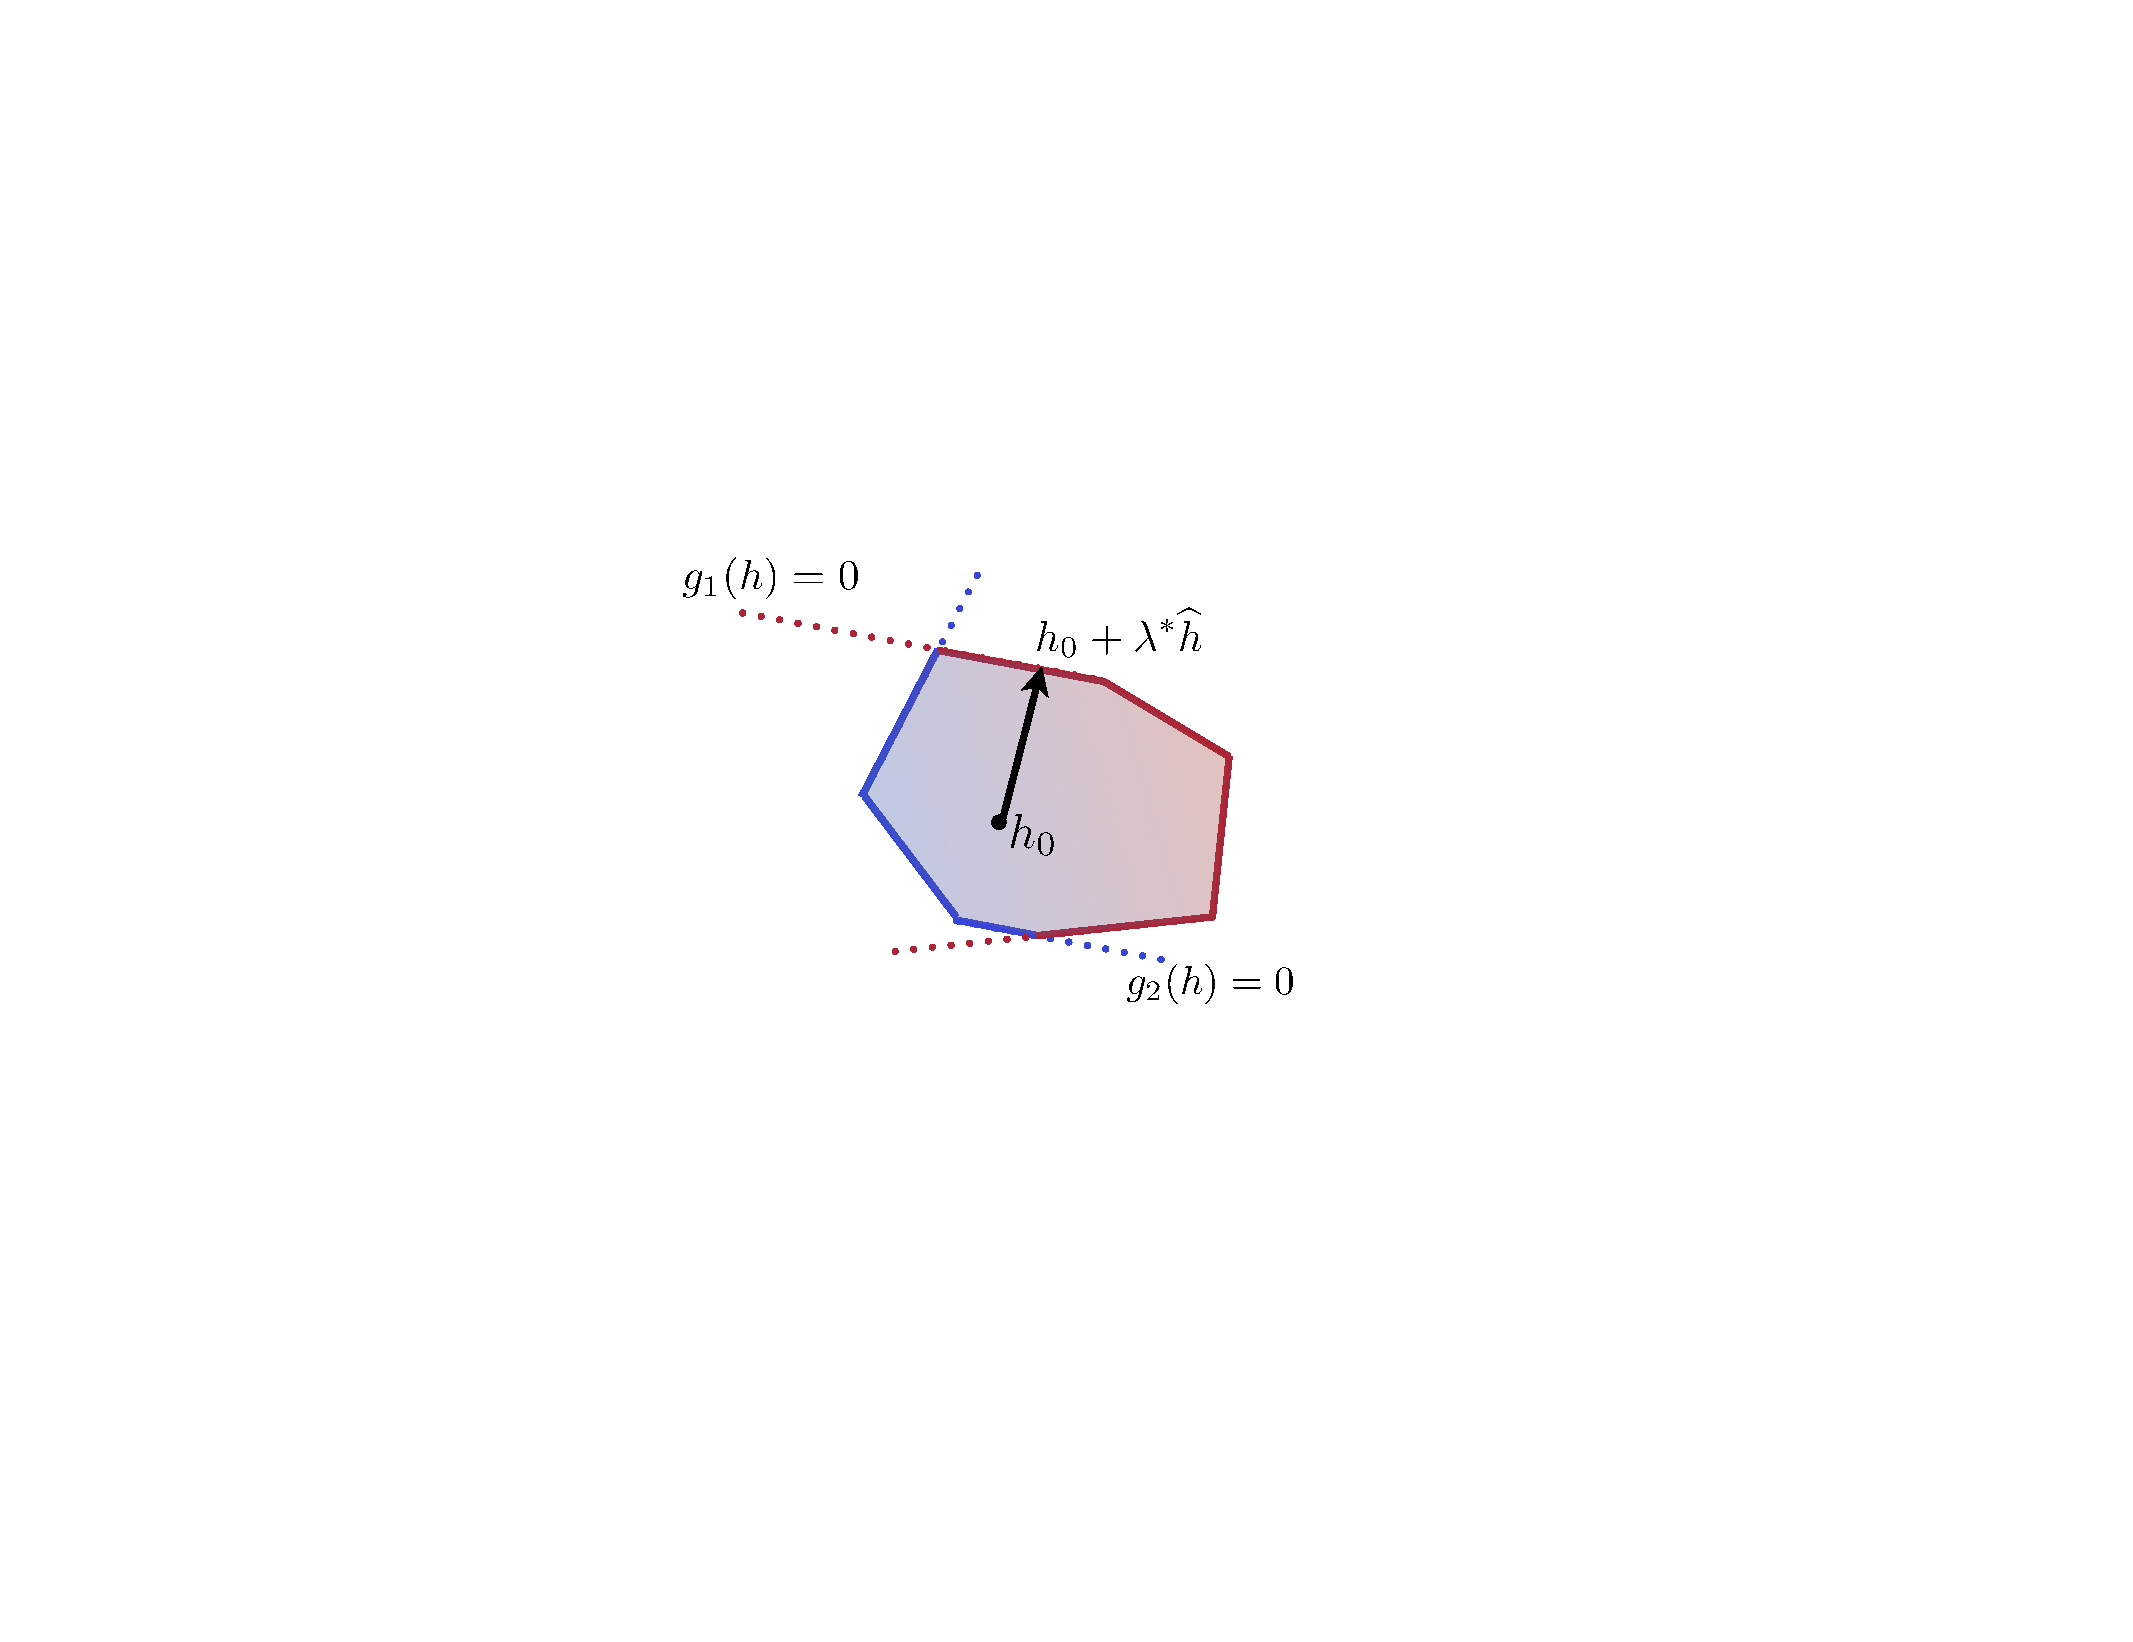
\includegraphics[scale=.30]{hsampling.pdf}
\caption{Illustration of the sampling process on the set $H''$.}
\label{fig:hsampling}
\end{figure}


\subsection{QP Formulation}
\label{sec:optimizationqp}

The SDP formulation described in the previous section is applicable
for a specific choice of $H''$. In this section, we present an
analysis that holds for an arbitrary compact, convex set $H''$. First, notice
that the problem of minimizing $G$ (expression \eqref{eq:optmaxmin}) is
related to the minimum enclosing ball (MEB) problem.  For a set
$D \subseteq \Rset^d$, the MEB problem is defined as follows:
\begin{equation*}
  \min_{\bu \in \Rset^d}\max_{\bv \in D} \|\bu - \bv\|^2.
\end{equation*}
Omitting the regularization and the $\min$ term from
\eqref{eq:optmaxmin} leads to a problem similar to the MEB.  Thus, we
could benefit from the extensive literature and algorithmic study
available for this problem
\citep{Kumar03,schonherr,Yildirim2008}.
However, to the best of our knowledge, there is currently no
solution available to this problem in the case of an infinite
set $D$, as in the case of our problem.
Instead, we present a solution for solving an approximation of
\eqref{eq:optmaxmin} based on sampling.

Let $\{h_1, \ldots, h_k\}$ be a set of hypotheses on the boundary of
$H''$, $\partial H''$
and let $\mathcal{C} = \mathcal{C}(h_1, \ldots, h_k)$ denote their
convex hull. The following is the sampling-based approximation of
\eqref{eq:optmaxmin} that we consider:
\begin{equation}
\label{eq:optmaxapp}
\min_{h \in \Hset} \lambda \norm{h}{K}^2 +
 \frac{1}{2} \max_{i=1,...,k} \cL_{\h P}(h, h_i) + \frac{1}{2}
 \min_{h' \in  \mathcal{C}} \cL_{\h P }(h, h').
\end{equation}

\begin{proposition}
\label{prop:dual}
Let $\mat Y =(Y_{ij}) \in \Rset^{n \times k}$ be the
matrix defined by $Y_{ij} = n^{-1/2} h_j(x_i')$ and
$\y' = (y'_1, \ldots, y'_k)^\top \in \Rset^k $ the vector defined by
$y'_i = n^{-1} \sum_{j=1}^n h_i(x'_j)^2$. Then, the dual problem of
\eqref{eq:optmaxapp} is given by
\begin{align}
\label{eq:dualapp}
\max_{\bm \alpha, \bm \gamma, \beta} & \ -\Big(\mat Y \bm \alpha + \frac{\bm
  \gamma}{2} \Big)^\top \Kt\Big(\lambda \I + \frac{1}{2}\Kt\Big)^{-1}
\Big(\mat Y \bm \alpha  + \frac{\bm \gamma}{2}\Big)
 - \frac{1}{2} \bm \gamma^\top \Kt \Kt^\dag \bm \gamma
+  \bm \alpha^\top \y' - \beta \\
\text{s.t.} & \ \1^\top \bm \alpha = \frac{1}{2}, \qquad  \1
\beta \geq -\mat Y^\top \bm \gamma, \qquad \bm \alpha\geq
0, \nonumber
\end{align}
where $\1$ is the vector in $\Rset^k$ with all components equal to
$1$. Furthermore, the solution $h$ of \eqref{eq:optmaxapp} can be
recovered from a solution $(\bm \alpha, \bm \gamma, \beta)$ of
\eqref{eq:dualapp} by $\forall x, h(x) =\sum_{i = 1}^n a_i K(x_i, x)$,
where $\bm a = \big(\lambda \I + \frac{1}{2}\Kt)^{-1}(\mat Y \bm
\alpha + \frac{1}{2}\bm \gamma)$.
\end{proposition}

The proof of the proposition is given in Appendix~\ref{app:qpformula}.
The result shows that, given a finite sample $h_1, \ldots, h_k$ on the
boundary of $H''$, \eqref{eq:optmaxapp} is in fact equivalent to a
standard QP. Hence, a solution can be found efficiently with one of
the many off-the-shelf algorithms for quadratic programming.

We now describe the process of sampling from the boundary of the set
$H''$, which is a necessary step for defining problem
\eqref{eq:optmaxapp}. We consider compact sets of the form
 $H'':= \{h'' \in \Hset \; | \; g_i(h'') \leq 0\}$, where the functions $g_i$
are continuous and convex. For instance, we could consider the set
$H''$ defined in the previous section. More generally, we can consider
a family of sets
$H''_p = \{h'' \in H | \; | \; \sum_{i=1}^m \qmin(x_i)|h(x_i) -y_i|^p
\leq r^p\}$.

Assume that there exists $h_0$ satisfying $g_i(h_0) < 0$. Our sampling
process is illustrated by Figure~\ref{fig:hsampling} and works as
follows: pick a random direction $\h h$ and define $\lambda_i$ to be
the minimal solution to the system
\begin{equation*}
  (\lambda \geq 0) \wedge (g_i(h_0 + \lambda \h{h}) = 0).
\end{equation*}
Set $\lambda_i = \infty$ if no solution is found and define
$\lambda^* = \min_i \lambda_i$. By the convexity and compactness of
$H''$ we can guarantee that $\lambda^* < \infty$. The hypothesis
$h =h_0 + \lambda^* \h h$ satisfies
$h \in H''$ and $g_j(h) = 0$ for $j$
such that $\lambda_j = \lambda^*$. The latter is straightforward. To
verify the former, assume that $g_i(h_0 + \lambda^* \h h) > 0$ for
some $i$. The continuity of $g_i$ would imply the existence of
$\lambda_i'$ with $0 < \lambda'_i < \lambda^* \leq \lambda _i$ such
that $g_i(h_0 + \lambda_i' \h h) = 0$. This would contradict the
choice of $\lambda_i$, thus, the inequality
 $g_i(h_0 + \lambda^* \h h) \leq 0$ must hold for all $i$.

Since a point $h_0$ with $g_i(h_0) < 0$ can be obtained by solving a
convex program and solving the equations defining $\lambda_i$ is, in
general, simple, the process described provides an efficient way of
sampling points from the convex set $H''$.

\subsection{Implementation for the \texorpdfstring{$L_2$}{L2} Loss}

We now describe how to fully implement our sampling-based algorithm
for the case where $L$ is equal to the $L_2$ loss.  In view of the
results of Section~\ref{sec:guarantees}, we let
$H'' = \{ h'' |\|h''\|_K \leq \Lambda \ \wedge \ \cL_{\qq}(h'', f_Q)
\leq r^2 \}$. We first describe the steps needed to find a point $h_0
\in H''$.  Let $h_\Lambda$ be such that $\|h_\Lambda\|_K = \Lambda$
and $\lambda_r \in \Rset_+$ be such that the solution $h_r$
 to the optimization problem
\begin{equation*}
 \min_{h \in \Hset} \lambda_r \| h \|^2 + \cL_{\qq}(h, f_Q),
\end{equation*}
satisfies $\cL_{\qq}(h_r, f_Q) = r^2$. It is easy to verify that the
existence of $\lambda_r$ is guaranteed for
$\min_{h \in H } \cL_\qq(h, f_Q) \leq r^2 \leq \sum_{i=1}^m \qq(x_i) y_i^2$.
 It is clear that the point $h_0 = \frac{1}{2} (h_r + h_\Lambda)$ is in
the interior of $H''$. Of course, finding $\lambda_r$ with the desired
properties is not straightforward. However, since $r$ is chosen via
validation, we do not need to find $\lambda_r$ as a function of
$r$. Instead, we can simply select $\lambda_r$ through
validation too.

In order to complete the sampling process, we must have an efficient
way of selecting a random direction $\h h$. If $H \subset \Rset^d$ is
a set of linear hypotheses, a direction $\h h$ can be sampled
uniformly by letting $\h h = \frac{\xi}{\| \xi \|}$, where $\xi$ is a
standard Gaussian random variable in $\Rset^d$. If $H$ is a subset of
a RKHS, by the representer theorem, we only need to consider
hypotheses of the form
$h = \sum_{i=1}^m \alpha_i K(x_i, \cdot)$. Therefore, we can sample a
direction $\h h = \sum_{i=1}^m \alpha'_i K(x_i, \cdot)$, where the
vector $\boldsymbol{\alpha'} = (\alpha'_1, \ldots, \alpha'_m)$ is
drawn uniformly from the unit sphere in $\Rset^m$.  A full
implementation of our algorithm thus consists of the following steps:
\begin{itemize}
\itemsep 0em
\item find the distribution
$\qmin = \argmin_{\qq \in \mathcal{Q}}   \dis(\qq, \h P)$. This can be
done by using the smooth approximation algorithm of
\cite{CortesMohri2013};
\item sample points from the set $H''$ using the sampling process
described above;
\item solve the QP introduced in Section~\ref{sec:optimizationqp}.
\end{itemize}

Notice that our algorithm only requires solving a simple QP and
therefore its complexity is the same as other adaptation algorithms
such as KMM, KLIEP and DM.

\section{Experiments}
\label{sec:experiments}

Here, we report the results of extensive comparisons between GDM and
several other adaptation algorithms which demonstrate the benefits of
our algorithm. We use the implementation described in the previous
section. The source code for our algorithm as well as all other
baselines described in this section can be found at
\url{http://cims.nyu.edu/~munoz}.
\begin{figure}[t]
\centering
\begin{tabular}{cc}
\raisebox{5pt}{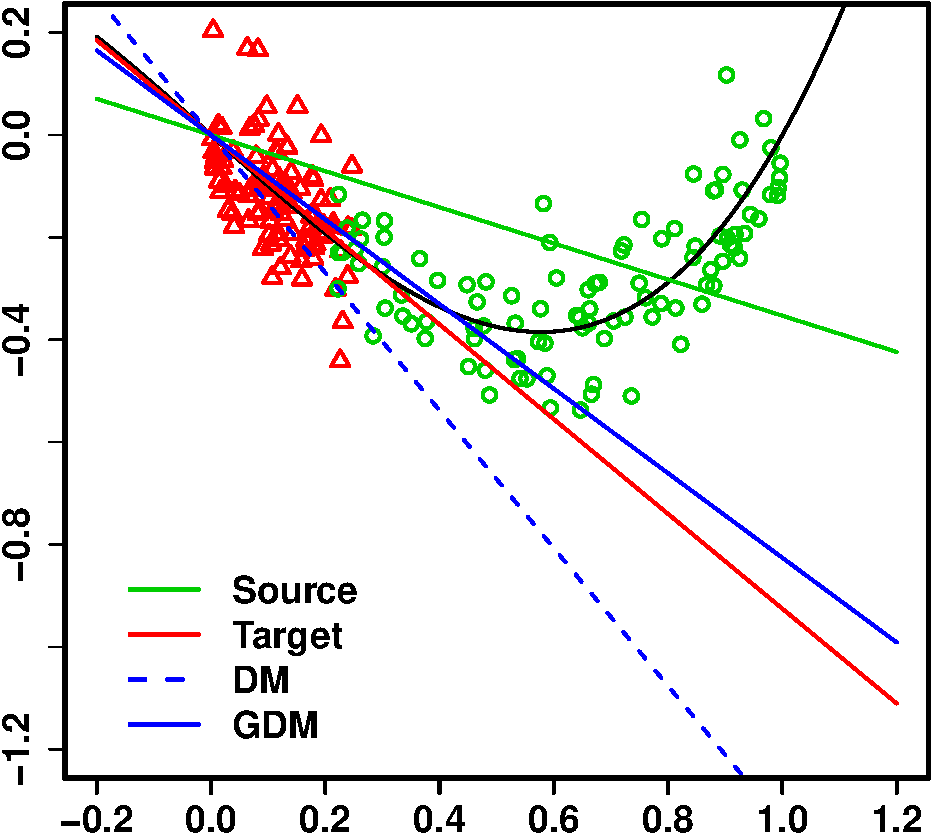
\includegraphics[scale=.20]{oned-crop.pdf}}
&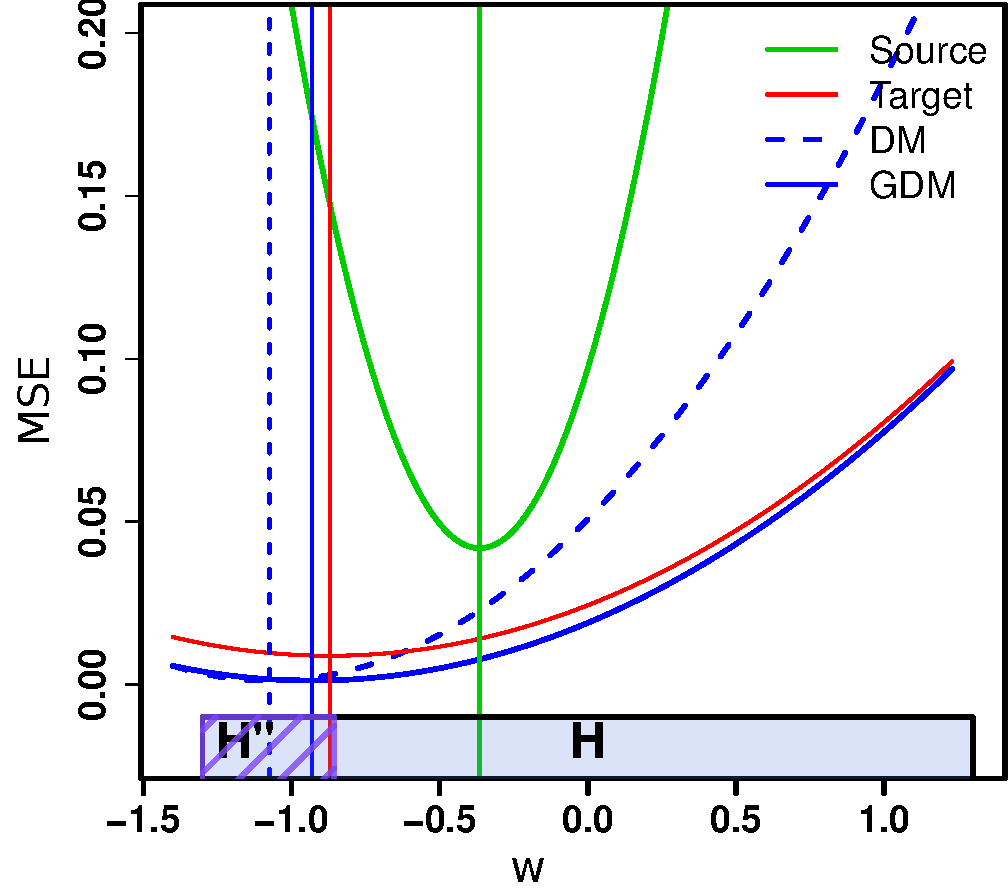
\includegraphics[scale=.20]{losses-crop.pdf}\\
(a)&(b)
\end{tabular}
\caption{(a) Hypotheses obtained by training on source
(green circles), target (red triangles) and using DM (dashed
blue) and GDM algorithms (solid blue). (b) Objective functions
for source and target distribution as well as  GDM and DM
algorithms. Sets $H$ and surrogate hypothesis set $H'' \subseteq H$
are shown at the bottom. The vertical lines represent the minimizing
hypothesis for each loss.}
\label{fig:classifiers}
\end{figure}

\subsection{Synthetic Data Set}

To compare the performances of the GDM and DM algorithms, we
considered the following synthetic one-dimensional task, which is
similar to the one considered by
\cite{HuangSmolaGrettonBorgwardtScholkopf2006}: the source domain
examples were sampled from the uniform distribution over the interval
$[.2, 1]$ and target ones sampled uniformly over $[0, .25]$. The
labels were given by the map $x \mapsto -x + x^3 + \xi$, where $\xi$
is a Gaussian random variable with mean $0$ and standard deviation
$0.1$. Our hypothesis set was defined by the family of linear
functions without an offset. Figure~\ref{fig:classifiers}(a) shows the
regression hypotheses obtained by training the DM and GDM algorithm as
well as those obtained by training on the source and target
distributions. The ideal hypothesis is shown in red.  Notice how the
GDM solution gives a closer approximation than DM to the ideal
solution.  In order to better understand the difference between the
solutions of these algorithms, Figure~\ref{fig:classifiers}(b) depicts the
objective function minimized by each algorithm as a function of the
slope $w$ of the linear function, the only variable of the
hypothesis. The vertical lines show the value of the minimizing
hypothesis for each loss. Keeping in mind that the regularization
parameter $\lambda$ used in ridge regression corresponds to a Lagrange
multiplier for the constraint $w^2 \leq \Lambda^2$ for some $\Lambda$
\citep{CortesMohri2013} [Lemma 1], the hypothesis set
$H = \{ w | w^2 \leq \Lambda^2\}$ is depicted at the bottom of this
plot.  The shaded region represents the set
$H'' = H \cap \{h'' |\cL_{\qmin} (h'') \leq r \}$. It is clear from
this plot that DM helps approximate the target loss
function. Nevertheless, only GDM seems to uniformly approach it. This
should come as no surprise since our algorithm was precisely designed
to achieve that.

\subsection{Adaptation Data Sets}

We now present the results of evaluating our algorithm against several
other adaptation algorithms. GDM is compared against DM and training
on the uniform distribution. The following baselines were also
used:

\begin{enumerate}
\itemsep 0em
 \item The KMM algorithm
\citep{HuangSmolaGrettonBorgwardtScholkopf2006}, which reweights
examples from the source distribution in order to match the mean of
the source and target data in a feature space induced by a universal
kernel. The hyper-parameters of this algorithm were set to the
recommended values of $B = 1000$ and
$\epsilon = \frac{\sqrt{m}}{\sqrt{m} - 1}$ .
\item KLIEP \citep{SugiyamaNakajimaKashimaVonBunauKawanabe2008}. This
algorithm estimates the importance ratio of the source and target
distribution by modeling this ratio as a mixture of basis functions
and learning the mixture coefficients from the data. Gaussian kernels
were used as basis functions for this algorithm and KMM. The bandwidth
for the kernel was selected from the set $\big \{\sigma d \colon
\sigma = 2^{-5} , \ldots, 2^5 \big\}$ via validation on the
\emph{test} set, where $d$ is the mean distance between points sampled
from the source domain.
\item FE \citep{daume2007frustratingly}. This algorithm maps source
and target data into a common high-dimensional feature space where the
difference of the distributions is expected to reduce.
\end{enumerate}

Since the two-stage algorithm of \cite{BickelBrucknerScheffer2007} was
already shown to perform similarly to KMM and KLIEP
\citep{CortesMohri2013}, for the sake of readability of our results,
we omitted the results of comparison with this algorithm. Finally, we
compare our algorithm with the ideal hypothesis $h^*$ returned by training
on the target sample $\cT$, which we denote by {\tt Tar}. Notice that
in practice, this is impossible as $\cT$ is unlabeled so we use this
result only to show the best attainable performance.

We selected the set of linear functions as our hypothesis set. The
learning algorithm used for all tasks was ridge regression and the
performance evaluated by the mean squared error. We follow the setup
of \cite{CortesMohri2011} and for all adaptation algorithms we
selected the parameter $\lambda$ via 10-fold cross validation over the
training data by using a grid search over the set of values
$\lambda \in \{2^{-10}, \ldots, 2^{10} \}$. The results of training on the
target distribution are presented for a parameter $\lambda$ tuned via
$10$-fold cross validation over the target data. We used the QP
implementation of our algorithm with the sampling set $H''$ and the
sampling mechanism defined at the end of
Section~\ref{sec:optimizationqp}, where the parameter $\lambda_r$ was
chosen from the same set as $\lambda$ via validation on a small
amount of data from the target distribution. Whereas there are other
methods such as transfer cross validation \citep{Zhong} to select the
parameters for our algorithm, these methods require the use of
importance weighting which as shown in \citep{importance} is not
theoretically justified.

\begin{figure}[t]
\centering
\begin{tabular}{cc}
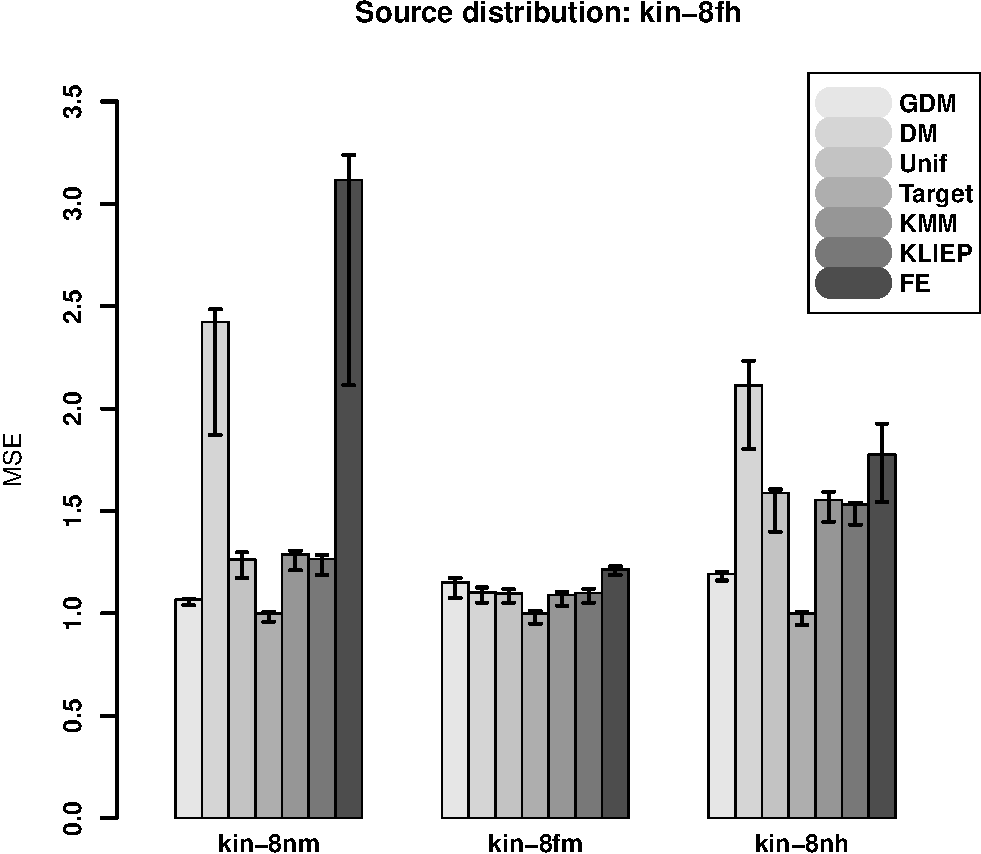
\includegraphics[width=2.1in, height=1.2in]{kin-crop.pdf}
&
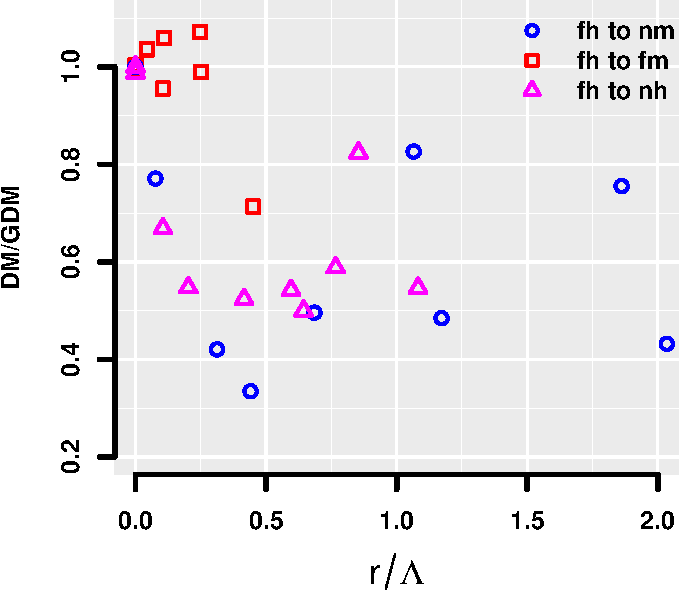
\includegraphics[width=1.9in, height=1.4in]{qtor.pdf} \\
(a) & (b)
\end{tabular}
\caption{(a)MSE performance for different adaptation algorithms when
  adapting from {\tt kin-8fh} to the three other {\tt kin-8xy}
  domains. (b) Relative error of DM over GDM as a function of the
  ratio $\frac{r}{\Lambda}$.}
\label{fig:kin}
\end{figure}

In order to achieve a fair comparison, all other algorithms were
allowed to use the small amount of labeled data too. Since, with the
exception of FE, all other baselines do not propose a way of dealing
with labeled data from the target distribution, we simply added this
data to the training set and ran the algorithms on the extended source
data as discussed in Section~\ref{sec:additional}.

The first task we considered is given by the 4 {\tt kin-8xy} Delve
data sets \citep{Delve}. These data sets are variations of the same
model: a realistic simulation of the forward dynamics of an 8 link
all-revolute robot arm. The task in all data sets consists of
predicting the distance of the end-effector from a target.  The data
sets differ by the degree of non-linearity (fairly linear, {\tts x=f},
or non-linear, {\tts x=n}) and the amount of noise in the output
(moderate, {\tts y=m}, or high, {\tts y=h}). The data set defines 4
different domains, that is 12 pairs of different distributions and
labeling functions. A sample of 200 points from each domain was used
for training and 10 labeled points from the target distribution were
used to select $H''$. The experiment was carried out 10 times and the
results of testing on a sample of $400$ points from the target domain
are reported in Figure~\ref{fig:kin}(a). The bars represent the median
performance of each algorithm. The error bars are the low and high
25\% quartiles respectively. All results were normalized in such a way
that the median performance of training on the source is equal to 1.
Notice that the performance of all algorithms is comparable when
adapting to {\tt kin8-fm} since both labeling functions are fairly
linear, yet only GDM is able to reasonably adapt to the two data sets
with different labeling functions. In order to better understand the
advantages of GDM over DM we plot the relative error of DM against GDM
as a function of the ratio $r / \Lambda$ in
Figure~\ref{fig:kin}(b), where $r$ is the radius defining $H''$ and
is selected through cross validation. Notice that when the ratio
$r / \Lambda$ is small then both algorithms behave similarly which is most
of the times for the adaptation task {\tts fh} to {\tts fm}. On the
other hand, a better performance of GDM can be obtained when the ratio
is larger. This is due to the fact that $r/\Lambda$ measures the
effective size of the set $H''$. A small ratio means that the size of
$H''$ is small and therefore the hypothesis returned by GDM will be
close to that of DM where as if $H''$ is large then GDM has the
possibility of finding  a better hypothesis.

\renewcommand{\arraystretch}{.8}
\begin{table}[t]
\vspace{.1in}
\begin{center}
\begin{tabular}{ccccccccc}
 \hline
  \multicolumn{8}{c}{\small{Task: Sentiment}} \\ \hline
\tiny{S} & \tiny{T} & \tiny{GDM} & \tiny{DM} & \tiny{Unif} &\tiny{Tar} & \tiny{KMM} & \tiny{KLIEP} & \tiny{F} \\  \hline
\multirow{3}{*}{ \tiny{B}} & \tiny{K} & $\mathbf{\scriptscriptstyle{ 0.763
    \pm ( 0.222 )}}$ & $\scriptscriptstyle{ 1.056   \pm ( 0.289 )}$ &
$\scriptscriptstyle{1.00}$ & $\scriptscriptstyle{ 0.517   \pm ( 0.152 )}$ & $\scriptscriptstyle{ 3.328   \pm ( 0.845 )}$ & $\scriptscriptstyle{ 3.494   \pm ( 1.144 )}$ & $\scriptscriptstyle{ 0.942   \pm ( 0.093 )}$\\
& \tiny{E} & $\mathbf{\scriptscriptstyle{ 0.574   \pm ( 0.211 )}}$ &
$\scriptscriptstyle{ 1.018   \pm ( 0.206 )}$ &$\scriptscriptstyle{1.00}$ & $\scriptscriptstyle{ 0.367   \pm ( 0.124 )}$ & $\scriptscriptstyle{ 3.018   \pm ( 0.319 )}$ & $\scriptscriptstyle{ 3.022   \pm ( 0.318 )}$ & $\scriptscriptstyle{ 0.857   \pm ( 0.135 )}$\\
& \tiny{D} & $\scriptscriptstyle{ 0.936   \pm ( 0.256 )}$ & $\scriptscriptstyle{
  1.215   \pm ( 0.255 )}$ & $\scriptscriptstyle{1.00}$ & $\scriptscriptstyle{ 0.623   \pm ( 0.152 )}$ & $\scriptscriptstyle{ 2.842   \pm ( 0.492 )}$ & $\scriptscriptstyle{ 2.764   \pm ( 0.446 )}$ & $\mathbf{\scriptscriptstyle{ 0.936   \pm ( 0.110 )}}$\\
\hline
 \multirow{3}{*}{ \tiny{K}} & \tiny{B} & $\mathbf{\scriptscriptstyle{
     0.854   \pm ( 0.119 )}}$ & $\scriptscriptstyle{ 1.258   \pm ( 0.117
   )}$& $\scriptscriptstyle{1.00}$ & $\scriptscriptstyle{ 0.665   \pm ( 0.085 )}$ & $\scriptscriptstyle{ 2.784   \pm ( 0.244 )}$ & $\scriptscriptstyle{ 2.642   \pm ( 0.218 )}$ & $\scriptscriptstyle{ 1.047   \pm ( 0.047 )}$\\
& \tiny{E} & $\scriptscriptstyle{ 0.975   \pm ( 0.131 )}$ & $\scriptscriptstyle{
  1.460   \pm ( 0.633 )}$ & $\scriptscriptstyle{1.00}$& $\scriptscriptstyle{ 0.653   \pm ( 0.201 )}$ & $\scriptscriptstyle{ 2.408   \pm ( 0.582 )}$ & $\scriptscriptstyle{ 2.157   \pm ( 0.255 )}$ & $\mathbf{\scriptscriptstyle{ 0.969   \pm ( 0.131 )}}$\\
& \tiny{D} & $\mathbf{\scriptscriptstyle{ 0.884   \pm ( 0.101 )}}$ & $\scriptscriptstyle{ 1.174   \pm ( 0.140 )}$ &$\scriptscriptstyle{1.00}$& $\scriptscriptstyle{ 0.665   \pm ( 0.071 )}$ & $\scriptscriptstyle{ 2.771   \pm ( 0.157 )}$ & $\scriptscriptstyle{ 2.620   \pm ( 0.210 )}$ & $\scriptscriptstyle{ 1.111   \pm ( 0.059 )}$\\
\hline
 \multirow{3}{*}{ \tiny{E}} & \tiny{B} & $\mathbf{\scriptscriptstyle{
     0.723   \pm ( 0.138 )}}$ & $\scriptscriptstyle{ 1.016   \pm ( 0.187 )}$
 & $\scriptscriptstyle{1.00}$& $\scriptscriptstyle{ 0.551   \pm ( 0.109 )}$ & $\scriptscriptstyle{ 3.433   \pm ( 0.694 )}$ & $\scriptscriptstyle{ 3.290   \pm ( 0.583 )}$ & $\scriptscriptstyle{ 1.035   \pm ( 0.059 )}$\\
& \tiny{K} & $\scriptscriptstyle{ 1.030   \pm ( 0.312 )}$ & $\scriptscriptstyle{
  1.277   \pm ( 0.283 )}$ & $\scriptscriptstyle{1.00}$& $\scriptscriptstyle{ 0.636   \pm ( 0.176 )}$ & $\scriptscriptstyle{ 2.173   \pm ( 0.249 )}$ & $\scriptscriptstyle{ 2.223   \pm ( 0.293 )}$ & $\mathbf{\scriptscriptstyle{ 0.955   \pm ( 0.199 )}}$\\
& \tiny{D} & $\mathbf{\scriptscriptstyle{ 0.731   \pm ( 0.171 )}}$ &
$\scriptscriptstyle{ 1.005   \pm ( 0.166 )}$ & $\scriptscriptstyle{1.00}$& $\scriptscriptstyle{ 0.518   \pm ( 0.117 )}$ & $\scriptscriptstyle{ 3.363   \pm ( 0.402 )}$ & $\scriptscriptstyle{ 3.231   \pm ( 0.483 )}$ & $\scriptscriptstyle{ 0.974   \pm ( 0.102 )}$\\
\hline
 \multirow{3}{*}{ \tiny{D}} & \tiny{B} & $\scriptscriptstyle{ 0.992   \pm
   ( 0.191 )}$ & $\scriptscriptstyle{ 1.026   \pm ( 0.090 )}$ &
 $\scriptscriptstyle{1.00}$& $\scriptscriptstyle{ 0.740   \pm ( 0.138 )}$ & $\scriptscriptstyle{ 2.571   \pm ( 0.616 )}$ & $\scriptscriptstyle{ 2.475   \pm ( 0.400 )}$ & $\mathbf{\scriptscriptstyle{ 0.986   \pm ( 0.041 )}}$\\
& \tiny{K} & $\mathbf{\scriptscriptstyle{ 0.870   \pm ( 0.212 )}}$ &
$\scriptscriptstyle{ 1.062   \pm ( 0.318 )}$ & $\scriptscriptstyle{1.00}$& $\scriptscriptstyle{ 0.557   \pm ( 0.137 )}$ & $\scriptscriptstyle{ 2.755   \pm ( 0.375 )}$ & $\scriptscriptstyle{ 2.741   \pm ( 0.347 )}$ & $\scriptscriptstyle{ 0.940   \pm ( 0.087 )}$\\
& \tiny{E} & $\mathbf{\scriptscriptstyle{ 0.674   \pm ( 0.135 )}}$ &
$\scriptscriptstyle{ 0.994   \pm ( 0.171 )}$ & $\scriptscriptstyle{1.00}$& $\scriptscriptstyle{ 0.478   \pm ( 0.098 )}$ & $\scriptscriptstyle{ 2.939   \pm ( 0.501 )}$ & $\scriptscriptstyle{ 2.878   \pm ( 0.418 )}$ & $\scriptscriptstyle{ 0.907   \pm ( 0.081 )}$\\
\hline
 \end{tabular}
\caption{ Adaptation from {\tt books} (B), {\tt kitchen} (K), {\tt
electronics} (E) and {\tt dvd} (D) to all other domains. Normalized
results: MSE of training on the unweighted source data is equal to
1. Results in bold represent the algorithm with the lowest MSE.}
\label{table:sent}
\end{center}
\end{table}

\begin{table}[t]
\vspace{.1in}
\centering
\begin{tabular}{ccccccccc}
 \hline
  \multicolumn{8}{c}{\small{Task: Images}} \\ \hline
\tiny{S} & \tiny{T} & \tiny{GDM} & \tiny{DM} & \tiny{Unif} & \tiny{Tar} & \tiny{KMM} & \tiny{KLIEP} & \tiny{F} \\  \hline
\multirow{3}{*}{ \tiny{C}} & \tiny{I} & $\mathbf{\scriptscriptstyle{ 0.927
    \pm ( 0.051 )}}$ & $\scriptscriptstyle{ 1.005   \pm ( 0.010 )}$ & $\scriptscriptstyle{1.00}$& $\scriptscriptstyle{ 0.879   \pm ( 0.048 )}$ & $\scriptscriptstyle{ 2.752   \pm ( 3.820 )}$ & $\scriptscriptstyle{ 0.936   \pm ( 0.016 )}$ & $\scriptscriptstyle{ 0.959   \pm ( 0.035 )}$\\
& \tiny{S} & $\scriptscriptstyle{ 0.938   \pm ( 0.064 )}$ & $\scriptscriptstyle{ 0.993   \pm ( 0.018 )}$ & $\scriptscriptstyle{1.00}$&$\scriptscriptstyle{ 0.840   \pm ( 0.057 )}$ & $\mathbf{\scriptscriptstyle{ 0.827   \pm ( 0.017 )}}$ & $\scriptscriptstyle{ 0.835   \pm ( 0.020 )}$ & $\scriptscriptstyle{ 0.947   \pm ( 0.025 )}$\\
& \tiny{B} & $\mathbf{\scriptscriptstyle{ 0.909   \pm ( 0.040 )}}$ & $\scriptscriptstyle{ 1.003   \pm ( 0.013 )}$ & $\scriptscriptstyle{1.00}$&$\scriptscriptstyle{ 0.886   \pm ( 0.052 )}$ & $\scriptscriptstyle{ 0.945   \pm ( 0.022 )}$ & $\scriptscriptstyle{ 0.942   \pm ( 0.017 )}$ & $\scriptscriptstyle{ 0.947   \pm ( 0.019 )}$\\
\hline
 \multirow{3}{*}{ \tiny{I}} & \tiny{C} & $\scriptscriptstyle{ 1.011   \pm
   ( 0.015 )}$ & $\mathbf{\scriptscriptstyle{ 0.951   \pm ( 0.011 )}}$ &
 $\scriptscriptstyle{1.00}$& $\scriptscriptstyle{ 0.802   \pm ( 0.040 )}$ & $\scriptscriptstyle{ 0.989   \pm ( 0.036 )}$ & $\scriptscriptstyle{ 1.009   \pm ( 0.042 )}$ & $\scriptscriptstyle{ 0.971   \pm ( 0.024 )}$\\
& \tiny{S} & $\scriptscriptstyle{ 1.006   \pm ( 0.030 )}$ & $\scriptscriptstyle{
  0.992   \pm ( 0.016 )}$ & $\scriptscriptstyle{1.00}$& $\scriptscriptstyle{ 0.871   \pm ( 0.030 )}$ & $\mathbf{\scriptscriptstyle{ 0.930   \pm ( 0.018 )}}$ & $\scriptscriptstyle{ 0.936   \pm ( 0.016 )}$ & $\scriptscriptstyle{ 0.973   \pm ( 0.017 )}$\\
& \tiny{B} & $\mathbf{\scriptscriptstyle{ 0.987   \pm ( 0.022 )}}$ &
$\scriptscriptstyle{ 1.009   \pm ( 0.010 )}$ & $\scriptscriptstyle{1.00}$& $\scriptscriptstyle{ 0.986   \pm ( 0.028 )}$ & $\scriptscriptstyle{ 1.011   \pm ( 0.028 )}$ & $\scriptscriptstyle{ 1.011   \pm ( 0.028 )}$ & $\scriptscriptstyle{ 0.994   \pm ( 0.018 )}$\\
\hline
 \multirow{3}{*}{ \tiny{S}} & \tiny{C} & $\scriptscriptstyle{ 1.022   \pm
   ( 0.037 )}$ & $\scriptscriptstyle{ 0.982   \pm ( 0.035 )}$ &
 $\scriptscriptstyle{1.00}$&  $\scriptscriptstyle{ 0.759   \pm ( 0.033 )}$ & $\scriptscriptstyle{ 1.172   \pm ( 0.043 )}$ & $\scriptscriptstyle{ 1.201   \pm ( 0.038 )}$ & $\mathbf{\scriptscriptstyle{ 0.938   \pm ( 0.036 )}}$\\
& \tiny{I} & $\mathbf{\scriptscriptstyle{ 0.924   \pm ( 0.049 )}}$ &
$\scriptscriptstyle{ 0.998   \pm ( 0.030 )}$ & $\scriptscriptstyle{1.00}$& $\scriptscriptstyle{ 0.831   \pm ( 0.047 )}$ & $\scriptscriptstyle{ 3.868   \pm ( 4.231 )}$ & $\scriptscriptstyle{ 1.227   \pm ( 0.039 )}$ & $\scriptscriptstyle{ 0.947   \pm ( 0.028 )}$\\
& \tiny{B} & $\mathbf{\scriptscriptstyle{ 0.898   \pm ( 0.072 )}}$ &
$\scriptscriptstyle{ 1.003   \pm ( 0.044 )}$ & $\scriptscriptstyle{1.00}$& $\scriptscriptstyle{ 0.821   \pm ( 0.053 )}$ & $\scriptscriptstyle{ 1.240   \pm ( 0.039 )}$ & $\scriptscriptstyle{ 1.248   \pm ( 0.041 )}$ & $\scriptscriptstyle{ 0.945   \pm ( 0.021 )}$\\
\hline
 \multirow{3}{*}{ \tiny{B}} & \tiny{C} & $\scriptscriptstyle{ 1.010   \pm
   ( 0.014 )}$ & $\mathbf{\scriptscriptstyle{ 0.956   \pm ( 0.017 )}}$ &
 $\scriptscriptstyle{1.00}$&  $\scriptscriptstyle{ 0.777   \pm ( 0.031 )}$ & $\scriptscriptstyle{ 1.028   \pm ( 0.033 )}$ & $\scriptscriptstyle{ 1.032   \pm ( 0.031 )}$ & $\scriptscriptstyle{ 0.980   \pm ( 0.019 )}$\\
& \tiny{I} & $\scriptscriptstyle{ 1.012   \pm ( 0.010 )}$ & $\scriptscriptstyle{
  1.004   \pm ( 0.007 )}$ &  $\scriptscriptstyle{1.00}$& $\scriptscriptstyle{ 0.966   \pm ( 0.009 )}$ & $\scriptscriptstyle{ 2.785   \pm ( 3.803 )}$ & $\mathbf{\scriptscriptstyle{ 0.981   \pm ( 0.018 )}}$ & $\scriptscriptstyle{ 1.000   \pm ( 0.004 )}$\\
& \tiny{S} & $\scriptscriptstyle{ 1.009   \pm ( 0.018 )}$ & $\scriptscriptstyle{ 0.988   \pm ( 0.010 )}$ &$\scriptscriptstyle{1.00}$& $\scriptscriptstyle{ 0.850   \pm ( 0.035 )}$ & $\mathbf{\scriptscriptstyle{ 0.930   \pm ( 0.022 )}}$ & $\scriptscriptstyle{ 0.934   \pm ( 0.024 )}$ & $\scriptscriptstyle{ 0.983   \pm ( 0.013 )}$\\
\hline
 \end{tabular}
\caption{ Adaptation from {\tt caltech256} (C), {\tt imagenet} (I),
  {\tt sun} (S) and {\tt bing} (B).}
\label{table:image}
\end{table}

For our next experiment we considered the cross-domain sentiment
analysis data set of \cite{Blitzer07Biographies}. This data set
consists of consumer reviews from 4 different domains: {\tt books,
  kitchen, electronics} and {\tt dvds}. We used the top 1000 uni-grams
and bi-grams as the features for this task. For each pair of
adaptation tasks we sampled $700$ points from the source distribution
and $700$ unlabeled points from the target. Only $50$ labeled points
from the target distribution were used to tune the parameter $r$ of
our algorithm. The final evaluation is done on a test set of $1000$
points. The mean results and standard deviations of this task are
shown in Table~\ref{table:sent} where the MSE values have been
normalized in such a way that the performance of training on the
source without reweighting is always 1.

Finally, we considered a novel domain adaptation task
\citep{TommasiTC14} of \linebreak
paramount importance in the computer vision
community. The domains correspond to 4 well known collections of
images: {\tt bing, caltech256, sun} and {\tt imagenet}. These data
sets have been standardized so that they all share the same feature
representation and labeling function \citep{TommasiTC14}. We sampled
800 labeled points from the source distribution and 800 unlabeled
points from the target distribution as well as 50 labeled target
points to be used for validation of $r$. The results of testing on
$1000$ points from the target domain are presented in
Table~\ref{table:image} where, again, the results were normalized
in such a way that the performance of training on the source data is
always 1.

After analyzing the results of this section we notice that the GDM
algorithm consistently outperforms DM and achieves similar or better
performance than all other common adaptation algorithms. It is worth
noticing that in some cases, other algorithms perform even worse than
training on the unweighted sample. This deficiency of the KLIEP
algorithm had already been pointed out by
\cite{SugiyamaNakajimaKashimaVonBunauKawanabe2008} but here we observe
that this problem can also affect the KMM algorithm. Finally, let us
point out that even though the FE algorithm also achieved performances
similar to GDM on the sentiment and image adaptation, its performance
was far from optimal adapting on the {\tt kin-8xy} task. Since there
is a lack of theoretical understanding for this algorithm, it is hard
to characterize the scenarios where FE would perform better than GDM.

\section{Conclusion}

We presented a new theoretically well-founded domain adaptation
algorithm seeking to minimize a less conservative quantity than the DM
algorithm. We presented an SDP solution for the particular case of the
$L_2$ loss which can be solved in polynomial time. Our empirical
results show that our new algorithm always performs better than or is
on par with the otherwise state-of-the-art DM algorithm. We also
provided tight generalization bounds for the domain adaptation problem
based on the $\cY$-discrepancy. As pointed out in
Section~\ref{sec:guarantees}, an algorithm that minimizes the
$\cY$-discrepancy would benefit from the best possible
guarantees. However, the lack of labeled data from the target
distribution makes this algorithm not viable. This suggests analyzing
a richer scenario where the learner is allowed to ask for a limited
number of labels from the target distribution. This setup, which is
related to active learning, seems to be in fact the closest one to
real-life applications and has started to receive attention from the
research community \citep{Berlind}. We believe that the discrepancy $\dis$ will
play a central role in the analysis of that scenario as well.

\section*{Acknowledgments}
We would like to thank the reviewers of KDD and JMLR for their
suggestions to improve this paper. This work was partly funded by the
NSF awards IIS-1117591 and CCF-1535987.

\appendix

\section{SDP Formulation}
\label{app:sdpdual}

\begin{lemma}
The Lagrangian dual of the problem
\begin{align}
\label{eq:maxprob2}
  \max_{\substack{\a \in \Rset^m \\ \|\Ks \a - \y\|^2 \leq r^2}}
& \ \frac{1}{2}\|\Kst \a\|^2 - \b^\top \Kt \Kst \a,
\end{align}
is given by
\begin{align*}
\min_{\eta \geq 0, \gamma} & \ \gamma \\
\text{s. t.} & \ \left(
\def\arraystretch{1.3}
\begin{array}{cc}
 -\frac{1}{2} \Kst^\top \Kst + \eta \Ks^2
& \frac{1}{2}\Kst^\top \Kt \b - \eta \Ks\y  \\
\frac{1}{2} \b^\top  \Kt \Kst - \eta \y^\top \Ks
&  \eta (\|\y\|^2 - r^2) + \gamma
\end{array}
\right) \succeq  0.
\end{align*}
Furthermore, the duality gap for these problems is zero.
\end{lemma}

\begin{proof}
For $\eta \geq 0$ the Lagrangian of \eqref{eq:maxprob2} is given by
\begin{align*}
  L(\a, \eta) & = \frac{1}{2}\|\Kst \a\|^2 - \b^\top \Kt \Kst \a
- \eta( \|\Ks \a - \y\|^2 - r^2) \\
& =\a^\top \Big(\frac{1}{2} \Kst^\top \Kst - \eta \Ks^2 \Big)
  \a +   (2 \eta \Ks \y - \Kst^\top \Kt \b )^\top  \a - \eta (\|\y\|^2
  - r^2).
\end{align*}
Since the Lagrangian is a quadratic function of $\a$ and that the
conjugate function of a quadratic can be expressed in terms of
the pseudo-inverse,
the dual is given by
\begin{align*}
  \min_{\eta \geq 0} & \ \frac{1}{4}(2 \eta \Ks \y - \Kst^\top \Kt
 \b)^\top \Big(\eta \Ks^2 - \frac{1}{2} \Kst^\top \Kst
 \Big)^{\dag}(2 \eta \Ks  \y - \Kst^\top \Kt \b) - \eta(\|\y\|^2 - r^2)\\
\text{s. t. } & \ \eta \Ks^2 - \frac{1}{2} \Kst^\top \Kst\succeq 0.
\end{align*}
Introducing the variable $\gamma$ to replace the objective
function yields the equivalent problem
\begin{flalign*}
\min_{\eta \geq 0, \gamma} & \gamma \\
\text{s. t. } & \ \eta \Ks^2 - \frac{1}{2} \Kst^\top \Kst \succeq
0 \\
& \gamma - \frac{1}{4} (2 \eta \Ks \y - \Kst^\top \Kt
  \b)^\top \Big(\eta \Ks^2 - \frac{1}{2}\Kst^\top \Kst\Big)^{\dag}
(2 \eta \Ks  \y - \Kst^\top \Kt \b) + \eta(\|\y\|^2 - r^2) \geq 0\\
\end{flalign*}
Finally, by the properties of the Schur complement
\citep{BoydVandenberghe2004}, the two constraints above are equivalent
to
\begin{equation*}
\left(
  \begin{array}{cc}
  -\frac{1}{2} \Kst^\top \Kst  + \eta \Ks^2
& \frac{1}{2} \Kst^\top  \Kt \b - \eta\Ks \y \\
\Big(\frac{1}{2} \Kst^\top  \Kt \b - \eta\Ks \y\Big)^\top
& \eta (\|\y\|^2 - r) + \gamma
\end{array}
\right) \succeq 0.
\end{equation*}
Since duality holds for a general QCQP with only one constraint
\citep{BoydVandenberghe2004}[Appendix B], the duality gap between
these problems is $0$.
\end{proof}

\begin{proposition}
The optimization problem \eqref{eq:kmaxmin} is equivalent to the
following SDP:
\begin{align*}
\max_{\alpha, \beta, \nu, \Z, \z} & \ \frac{1}{2} \Tr(\Kst^\top \Kst \Z)
- \beta - \alpha\\
\text{s. t} & \ \left(
\def\arraystretch{1.3}
\begin{array}{cc}
\nu \Ks^2 + \frac{1}{2}\Kst^\top \Kst - \frac{1}{4} \wt{\mat K}
& \nu  \Ks \y + \frac{1}{4}\wt{\mat K} \z \\
\nu  \y^\top \Ks + \frac{1}{4} \z^\top \wt{\mat K}
&\alpha + \nu (\|\y\|^2 - r^2)
\end{array}
\right) \succeq 0 \quad \wedge \quad
\left(
\begin{array}{cc}
\Z & \z \\
\z^\top & 1
\end{array}
\right) \succeq 0 \\
& \ \left(
\def\arraystretch{1.3}
\begin{array}{cc}
\lambda \Kt + \Kt^2 & \frac{1}{2} \Kt \Kst \z \\
\frac{1}{2} \z^\top \Kst^\top \Kt & \beta
\end{array}
\right) \succeq 0
\; \wedge \; \Tr(\Ks^2 \Z) - 2\y^\top \Ks \z + \|\y\|^2 \leq r^2
\; \wedge \; \nu \geq 0,
\end{align*}
where $\wt{\mat K} = \Kst^\top \Kt (\lambda \Kt + \Kt^2)^\dag \Kt \Kst$.
\end{proposition}

\begin{proof}

By Lemma~\ref{lemma:sdpdual}, we may rewrite
\eqref{eq:kmaxmin} as
\begin{align}
\label{eq:firstequiv}
  \min_{\a, \gamma , \eta, \b}
 & \ \b^\top (\lambda \Kt + \Kt^2) \b + \frac{1}{2}
   \a^\top   \Kst^\top \Kst \a - \a^\top  \Kst^\top \Kt \b + \gamma \\
\text{s. t. } & \
 \left(
\def\arraystretch{1.3}
\begin{array}{cc}
 -\frac{1}{2} \Kst^\top \Kst + \eta \Ks^2  &
 \frac{1}{2}\Kst^\top \Kt \b - \eta \Ks \y \\
\frac{1}{2} \b^\top  \Kt \Kst - \eta \y^\top \Ks &
 \eta (\|\y\|^2 - r^2) + \gamma
\end{array}
\right)  \quad \wedge \quad \eta \geq 0 \nonumber \\
& \ \|\Ks \a - \y\|^2 \leq r^2. \nonumber
\end{align}
Let us apply the change of variables
$\b = \frac{1}{2}(\lambda \Kt + \Kt^2)^{\dag} \Kt \Kst \a +\v$.
The following equalities can be easily verified.
\begin{align*}
\b^\top (\lambda \Kt + \Kt^2) \b
&  = \frac{1}{4} \a^\top \Kst^\top \Kt (\lambda \Kt + \Kt^2)^\dag \Kt \Kst \a + \v^\top \Kt \Kst \a + \v^\top (\lambda \Kt + \Kt^2) \v.\\
\a^\top \Kst^\top  \Kt \b
& = \frac{1}{2} \a^\top \Kst^\top \Kt (\lambda \Kt + \Kt^2)^\dag \Kt \Kst \a + \v^\top \Kt \Kst \a.
\end{align*}
Thus, replacing $\b$ on \eqref{eq:firstequiv} yields
\begin{align*}
  \min_{\a, \v, \gamma , \eta}
 & \ \v^\top (\lambda \Kt + \Kt^2) \v + \
   \a^\top \Big(\frac{1}{2} \Kst^\top \Kst
   - \frac{1}{4}\wt{\mat K} \Big)\a + \gamma\\
\text{s. t. } & \
 \left(
\def\arraystretch{1.3}
\begin{array}{cc}
 -\frac{1}{2} \Kst^\top \Kst + \eta \Ks^2
& \frac{1}{4} \wt{\mat K}\a + \frac{1}{2}\Kst^\top \Kt \v - \eta \Ks \y \\
\frac{1}{4} \a^\top \wt{\mat K} + \frac{1}{2}\v^\top \Kt \Kst
- \eta \y^\top \Ks
& \eta (\|\y\|^2 - r^2) + \gamma
\end{array}
\right) \succeq 0  \quad \wedge \quad \eta \geq 0 \nonumber \\
& \ \|\Ks \a - \y\|^2 \leq r^2. \nonumber
\end{align*}
Introducing the scalar multipliers $\mu, \nu \geq 0$ and the matrix
\begin{equation*}
\left(
\begin{array}{cc}
\Z & \z \\
\z^\top & \wt z,
\end{array}
\right) \succeq 0
\end{equation*}
as a multiplier for the matrix constraint, we can form the Lagrangian:
\begin{multline*}
\mathfrak{L} := \v^\top (\lambda \Kt + \Kt^2) \v
+ \a^\top \Big(\frac{1}{2} \Kst^\top \Kst - \frac{1}{4}\wt{\mat K} \Big)\a
+ \gamma - \mu \eta + \nu (\|\Ks \a - \y\|^2 - r^2) \\
- \Tr  \left( \left(
\begin{array}{cc}
\Z & \z \\
\z & \wt z
\end{array}
\right)
\left(
\def\arraystretch{1.3}
\begin{array}{cc}
 -\frac{1}{2} \Kst^\top \Kst + \eta \Ks^2
& \frac{1}{4} \wt{\mat K}\a + \frac{1}{2}\Kst^\top \Kt \v - \eta \Ks \y \\
\frac{1}{4} \a^\top \wt{\mat K} + \frac{1}{2}\v^\top \Kt \Kst
- \eta \y^\top \Ks
& \eta (\|\y\|^2 - r^2) + \gamma
\end{array}
\right) \right).
\end{multline*}
The KKT conditions $\frac{\partial \mathfrak L}{\partial \eta} =
\frac{\partial \mathfrak L}{\partial \gamma} = 0$ trivially imply
$\wt z= 1$ and
$\Tr(\Ks^2 \Z) - 2\y^\top \Ks \z + \|\y\|^2 - r^2 + \mu = 0$.
These constraints on the dual variables guarantee that the primal
variables $\eta$ and $\gamma$ will vanish from the Lagrangian, thus
yielding
\begin{multline*}
\mathfrak{L} = \frac{1}{2} \Tr(\Kst^\top \Kst \Z) + \nu(\|\y\|^2 - r^2)
+ \v^\top (\lambda \Kt + \Kt^2) \v^\top - \z^\top \Kst^\top \Kt \v\\
+ \a^\top\Big(\nu \Ks^2 + \frac{1}{2}\Kst^\top \Kst - \frac{1}{4} \wt{\mat K}\Big) \a -\Big(2 \nu  \Ks \y + \frac{1}{2}\wt{\mat K} \z\Big)^\top \a.
\end{multline*}
This is a quadratic function on the primal variables $\a$ and $\v$
with minimizing solutions
\begin{equation*}
\a = \frac{1}{2} \Big(\nu \Ks^2 + \frac{1}{2}\Kst^\top \Kst - \frac{1}{4} \wt{\mat K}\Big)^\dag \Big(2 \nu  \Ks \y + \frac{1}{2}\wt{\mat K} \z\Big)
\qquad \text{and} \qquad
\v = \frac{1}{2}(\lambda \Kt +  \Kt^2)^{\dag}\Kt \Kst \z,
\end{equation*}
and optimal value equal to the objective of the Lagrangian dual:
\begin{multline*}
 \frac{1}{2} \Tr(\Kst^\top \Kst \Z) + \nu(\|\y\|^2 - r^2)
- \frac{1}{4} \z^\top \wt{\mat K} \z  \\
- \frac{1}{4} \Big(2 \nu  \Ks \y + \frac{1}{2}\wt{\mat K} \z\Big)^\top
\Big(\nu \Ks^2 + \frac{1}{2}\Kst^\top \Kst - \frac{1}{4} \wt{\mat K}\Big)^\dag
\Big(2 \nu  \Ks \y + \frac{1}{2}\wt{\mat K} \z\Big).
\end{multline*}
As in Lemma~\ref{lemma:sdpdual}, we apply the properties of the Schur
complement to show that the dual is given by
\begin{align*}
\max_{\alpha, \beta, \nu, \Z, \z} & \ \frac{1}{2} \Tr(\Kst^\top \Kst \Z)
- \beta - \alpha\\
\text{s. t} & \ \left(
\def\arraystretch{1.3}
\begin{array}{cc}
\nu \Ks^2 + \frac{1}{2}\Kst^\top \Kst - \frac{1}{4} \wt{\mat K}
& \nu  \Ks \y + \frac{1}{4}\wt{\mat K} \z\  \\
\nu \y^\top  \Ks + \frac{1}{4} \z^\top \wt{\mat K}
&\alpha + \nu (\|\y\|^2 - r^2)
\end{array}
\right) \succeq 0 \quad \wedge \quad
\left(
\begin{array}{cc}
\Z & \z \\
\z^\top & 1
\end{array}
\right) \succeq 0 \\
& \ \Tr(\Ks^2 \Z) - 2\y^\top \Ks \z + \|\y\|^2 \leq r^2
\quad \wedge \quad \beta \geq \frac{1}{4} \z^\top \wt{\mat K} \z
\quad \wedge \quad \nu \geq 0.
\end{align*}
Finally, recalling the definition of $\wt{\mat K}$ and using the
Schur complement one more time we arrive to the final SDP formulation
\begin{align*}
\max_{\alpha, \beta, \nu, \Z, \z} & \ \frac{1}{2} \Tr(\Kst^\top \Kst \Z)
- \beta - \alpha\\
\text{s. t} & \ \left(
\def\arraystretch{1.3}
\begin{array}{cc}
\nu \Ks^2 + \frac{1}{2}\Kst^\top \Kst - \frac{1}{4} \wt{\mat K}
& \nu  \Ks \y + \frac{1}{4}\wt{\mat K} \z \\
\nu  \y^\top \Ks + \frac{1}{4} \z^\top \wt{\mat K}
&\alpha + \nu (\|\y\|^2 - r^2)
\end{array}
\right) \succeq 0 \quad \wedge \quad
\left(
\begin{array}{cc}
\Z & \z \\
\z^\top & 1
\end{array}
\right) \succeq 0 \\
& \ \left(
\def\arraystretch{1.3}
\begin{array}{cc}
\lambda \Kt + \Kt^2 & \frac{1}{2} \Kt \Kst \z \\
\frac{1}{2} \z^\top \Kst^\top \Kt & \beta
\end{array}
\right) \succeq 0
\; \wedge \; \Tr(\Ks^2 \Z) - 2\y^\top \Ks \z + \|\y\|^2 \leq r^2
\; \wedge \; \nu \geq 0.
\end{align*}
\end{proof}

\section{QP  Formulation}
\label{app:qpformula}

\begin{proposition}
Let $\mat Y =(Y_{ij}) \in \Rset^{n \times k}$ be the
matrix defined by
$Y_{ij} = n^{-1/2} h_j(x_i')$ and $\y' = (y'_1,\ldots, y'_k)^\top \in \Rset^k $
the vector defined by $y'_i = n^{-1}\sum_{j=1}^n h_i(x'_j)^2$.
Then, the dual problem of \eqref{eq:optmaxapp} is given by
\begin{align}
\label{eq:dual}
\max_{\bm \alpha, \bm \gamma, \beta} & \ -\Big(\mat Y \bm \alpha + \frac{\bm
  \gamma}{2} \Big)^\top \Kt\Big(\lambda \I + \frac{1}{2}\Kt\Big)^{-1}
\Big(\mat Y \bm \alpha  + \frac{\bm \gamma}{2}\Big)
-\frac{1}{2} \bm \gamma^\top \Kt \Kt^\dag \bm \gamma +
\bm \alpha^\top \y' - \beta\\
\text{s.t.} & \ \1^\top \bm \alpha = \frac{1}{2}, \qquad  \1
\beta \geq -\mat Y^\top \bm \gamma, \qquad \bm \alpha\geq
0, \nonumber
\end{align}
where $\1$ is the vector in $\Rset^k$ with all components equal to
$1$. Furthermore, the solution $h$ of \eqref{eq:optmaxapp} can be
recovered from a solution $(\bm \alpha, \bm \gamma, \beta)$ of
\eqref{eq:dual} by $\forall x, h(x) =\sum_{i = 1}^n a_i K(x_i, x)$,
where $\bm a = \big(\lambda \I + \frac{1}{2}\Kt)^{-1}(\mat Y \bm
\alpha + \frac{1}{2}\bm \gamma)$.
\end{proposition}

We will first prove a simplified version of the proposition for the
case of linear hypotheses, i.e. we can represent hypotheses in $\Hset$
and elements of $\cX$ as vectors $\w, \x \in \Rset^d$
respectively. Define $\X' = n^{-1/2} (\x_1', \ldots, \x_n')$ to be the
matrix whose columns are the normalized sample points from the target
distribution. Let also $\{\w_1, \ldots, \w_k\}$ be a sample taken from
$\partial H''$ and define
$\bm W := (\w_1, \ldots, \w_k) \in \Rset^{d  \times k}$.
 Under this notation, problem \eqref{eq:optmaxapp} may be
rewritten as
\begin{equation}
\label{eq:linoptimization}
\min_{\w \in \Rset^d} \lambda \|\w\|^2 + \frac{1}{2} \max_{i =1,
  \dots, k} \|\X'^\top(\w - \w_i)\|^2 + \frac{1}{2} \min_{\w' \in
  \mathcal C} \|\X'^\top (\w - \w')\|^2.
\end{equation}

\begin{lemma}
The Lagrange dual of problem \eqref{eq:linoptimization} is given by
\begin{align*}
\max_{\bm \alpha, \bm \gamma, \beta}& -\Big(\mat Y \bm \alpha \!+\! \frac{\bm \gamma}{2}\Big)^\top
\X'^\top \Big(\lambda \I \!+\! \frac{\X' \X'^\top}{2}\Big)^{-1}\X' \Big(\bm
Y \bm\alpha \!+\! \frac{\bm \gamma}{2}\Big)
- \frac{1}{2}\bm \gamma^\top \X'^\top (\X' \X'^\top)^\dag
\X' \bm \gamma + \bm \alpha^\top \y' - \beta\\
\text{s. t.} & \ \1^\top \bm \alpha = \frac{1}{2} \quad \quad  \1
\beta \geq- \mat Y^\top \bm \gamma \quad \quad \bm \alpha\geq
0,
\end{align*}
where $\mat Y = \X'^\top \bm W$ and $\y'_i =\|\X'^\top \w_i\|^2$.
\end{lemma}

\begin{proof}
By applying the change of variable $\bu = \w' - \w$, problem
\eqref{eq:linoptimization} is can be made equivalent to
\begin{equation*}
  \min_{\w \in \Rset^d \bu \in \mathcal{C} - \w} \lambda \|\w\|^2 +
\frac{1}{2} \|\X'^\top \w\|^2 + \frac{1}{2}\|\X'^\top \bu\|^2 +
\frac{1}{2}\max_{i=1,\ldots, k} \|\bm \X'^\top \w_i\|^2 -2 \w_i^ \top
\X' \X'^\top \w.
\end{equation*}
By making the constraints on $\bu$ explicit and replacing the
maximization term with the variable $r$ the above problem becomes
\begin{align*}
  \min_{\w, \bu , r, \bm \mu}
& \quad \lambda \|\w\|^2 +   \frac{1}{2}
  \|\X'^\top  \w\|^2 +  \frac{1}{2}\|\X'^\top \bu\|^2 + \frac{1}{2}r \\
\text{s. t.}
& \quad \1 r \geq \y' - 2 \mat Y^\top \X'^\top  \w
\quad \wedge \quad \1^\top \bm \mu =1
\quad \wedge \quad \bm \mu \geq 0
\quad \wedge \quad \bm W \bm \mu - \w = \bu.
\end{align*}
For $\bm \alpha, \bm \delta \geq 0$, the Lagrangian of this problem is
defined as
\begin{align*}
\mathfrak{L}(\w, \bu, \bm \mu, r, \bm \alpha, \beta, \bm \delta, \bm \gamma')
& = \lambda \|\w\|^2 +   \frac{1}{2}  \|\X'^\top  \w\|^2
+ \frac{1}{2}\|\X'^\top \bu\|^2 + \frac{1}{2}r  + \beta(\1^\top  \bm \mu - 1)\\
&+ \bm \alpha^\top(\y' - 2(\X' \mat Y)^\top \w - \1 r)
- \bm \delta^\top \bm \mu + \bm \gamma'^\top(\bm W \bm  \mu - \w - \bu).
\end{align*}
Minimizing with respect to the primal variables yields the following
KKT conditions:
\begin{align}
  \1^\top \bm \alpha = \frac{1}{2} & \quad \quad
  \1\beta  = \bm \delta -\bm W^\top \bm \gamma'. \label{eq:linear}\\
\label{eq:quad}
  \bm \X'\X'^\top \bu = \bm \gamma' & \quad \quad
 2 \left(\lambda \I + \frac{\X' \X'^\top}{2}\right)\w = 2(\X' \bm
 Y)\bm \alpha + \bm \gamma'.
\end{align}
Condition \eqref{eq:linear} implies that the terms involving $r$
and $\bm \mu$ will vanish from the Lagrangian. Furthermore, the first
equation in \eqref{eq:quad} implies that any feasible $\bm \gamma'$
must satisfy $\bm \gamma' = \X' \bm \gamma$ for some $\gamma \in
\Rset^n$. Finally, it is immediate that $\bm \gamma'^\top \bu =
\bu^\top \X' \X'^\top \bu$ and $2\w ^\top\left(\lambda \I + \frac{\X'
\X'^\top}{2}\right) \w = 2 \bm \alpha^\top (\X' \mat Y)^\top \w \bm
+ \bm \gamma'^\top \w$. Thus, at the optimal point, the Lagrangian
becomes
 \begin{align*}
&  \quad  -\w^\top \Big(\lambda \I + \frac{1}{2} \X' \X'^\top\Big) \w
- \frac{1}{2} \bu^\top  \X' \X'^\top  \bu + \bm \alpha^\top \y' - \beta \\
\text{s. t.}
& \quad \1^\top \bm \alpha = \frac{1}{2} \quad \quad  \1
\beta = \bm \delta - \bm W^\top  \bm \gamma' \quad \quad \bm \alpha\geq 0 \wedge
\bm \delta \geq 0.
 \end{align*}
The positivity of $\bm \delta$ implies that
$\1\beta \geq -\bm W^\top \bm \gamma'$. Solving for $\w$ and $\bu$ on
\eqref{eq:quad} and applying the change of variable
$\X' \bm \gamma = \bm\gamma'$ we obtain the final expression for the
dual problem:
\begin{align*}
\max_{\bm \alpha, \bm \gamma, \beta}
& -\Big(\mat Y \bm \alpha \!+\! \frac{\bm \gamma}{2}\Big)^\top
\X'^\top \Big(\lambda \I \!+\! \frac{\X' \X'^\top}{2}\Big)^{-1}\X' \Big(\bm
Y \bm\alpha \!+\! \frac{\bm \gamma}{2}\Big)
- \frac{1}{2}\bm \gamma^\top \X'^\top (\X' \X'^\top)^\dag
\X' \bm \gamma + \bm \alpha^\top \y' - \beta\\
\text{s. t.}
& \ \1^\top \bm \alpha = \frac{1}{2} \quad \quad  \1
\beta \geq- \mat Y^\top \bm \gamma \quad \quad \bm \alpha\geq 0,
\end{align*}
where we have used the fact that
 $\mat Y^\top \bm \gamma = \W \X'^\top \bm \gamma$
to simplify the constraints. Notice also that we can
recover the solution $\w$ of problem \eqref{eq:linoptimization} as
$\w = (\lambda \I + \frac{1}{2} \X'^\top \X')^{-1}\X'( \mat Y \bm \alpha +
\frac{1}{2}\bm \gamma)$
\end{proof}

The proof of Proposition~\ref{prop:dual} follows from a
straightforward application of the well known matrix identities
$ \X'(\lambda \I + \X'^\top \X')^{-1}
 =(\lambda \I + \X'\X'^\top)^{-1} \X'$
 and $\X'^\top \X' (\X'^\top \X')^\dag
=  \X'^\top (\X' \X'^\top) ^\dag \X'$,
 and by the fact that the kernel matrix $\Kt$ is equal to
$\X'^\top \X'$.

\section{\texorpdfstring{$\mu$}{mu}-admissibility}
\label{app:muadmissible}

\begin{lemma}
\label{lemma:muadmissible}
Assume that $L_p(h(x), y) \leq M$ for all $x \in \cX$ and $y \in \cY$,
then $L_p$ is $\mu$-admissible with $\mu = p M^{p - 1}$.
\end{lemma}

\begin{proof}
Since $x \mapsto x^p$ is $p$-Lipschitz over $[0,1]$ we can write
\begin{align*}
| L(h(x),y) - L(h'(x), y) |
& = M^p \bigg|\Big(\frac{|h(x) - y|}{M}\Big)^p  -
\Big(\frac{|h'(x) - y|}{M}\Big)^p \bigg|\\
& \leq p M^{p-1}|h(x) - y + y - h'(x)|  = p M^{p-1} |h(x) - h'(x)|.
\end{align*}
%which concludes the proof.
\end{proof}

\begin{lemma}
\label{lemma:holder}
Let $L$ be the $L_p$ loss for some $p \geq 1$ and let $h, h', h''$ be
functions satisfying $L_p(h(x), h'(x)) \leq M$ and
$L_p(h''(x), h'(x)) \leq M$ for all $x \in \cX$, for some $M \geq 0$.
Then, for any distribution $\cD$ over $\cX$, the following inequality holds:
\begin{equation}
| \cL_\cD(h, h') - \cL_\cD(h'', h') | \leq p M^{p-1}[\cL_\cD(h, h'')]^{\frac{1}{p}}.
\end{equation}
\end{lemma}

\begin{proof}
Proceeding as in the proof of Lemma~\ref{lemma:muadmissible}, we obtain
\begin{align*}
| \cL_\cD(h, h') - \cL_\cD(h'', h') |
& = | \E_{x \in \cD}\big[L_p(h(x),
h'(x)) - L_p(h''(x), h'(x)\big]  |  \\
& \leq p M^{p-1} \E_{x \in \cD} \big[|h(x) - h''(x)| \big].
\end{align*}
Since $p \geq 1$, by Jensen's inequality, we can write $\E_{x \in \cD}
\big[|h(x) - h''(x)| \big] \leq \E_{x \in \cD} \big[|h(x) - h''(x)|^p
\big]^{1/p} = [\cL_\cD(h, h'')]^{\frac{1}{p}}$.
\end{proof}
%\bibliographystyle{natbib}
\bibliography{daj}
\end{document}
